% Manuscript entry. The two opening sections are the original source files.
\pdfminorversion=7
\pdfmapfile{+symbols.map}
\pdfmapfile{+cm.map}
\pdfmapfile{+cmextra.map}
\documentclass[sigconf,nonacm]{acmart}
\usepackage{pvldb}
\settopmatter{printacmref=false,printfolios=true}
\usepackage{booktabs,multirow,array,makecell}
\let\Bbbk\relax
\usepackage{amsmath,amssymb}
\usepackage{graphicx,subfigure}
\usepackage{needspace,placeins,pifont,xspace,xstring}
\usepackage[ruled,vlined,linesnumbered]{algorithm2e}
\usepackage{cleveref}
\setlength{\subfigcapskip}{1pt}
\setcounter{dbltopnumber}{3}
\renewcommand{\topfraction}{0.92}
\renewcommand{\dbltopfraction}{0.95}
\renewcommand{\textfraction}{0.07}
\renewcommand{\floatpagefraction}{0.8}
\renewcommand{\dblfloatpagefraction}{0.60}
\newcommand{\LIMIT}{\textsf{LIMIT}\xspace}
\newcommand{\qpm}[2]{#1\,{\scriptsize$\pm$#2}}
\newcommand{\stitle}[1]{\vspace{1ex}\noindent\textbf{#1}}
\newcommand{\cmark}{\ding{51}}
% Default path: evidence off, no input shuffle.
% The objective is estimated merge input tokens; no unverified cost formula is used.
% Full materializes each pass. LIMIT pulls the same groups and stops at K.
% h=1 is LT(h), not a second family.
\DontPrintSemicolon
\newcommand{\Rank}{\mbox{\textsc{ListwiseRank}}}
\newcommand{\Replay}{\mbox{\textsc{Replay}}}
\newcommand{\Refresh}{\mbox{\textsc{Refresh}}}
\newcommand{\MergeGroup}{\mbox{\textsc{MergeGroup}}}
\newcommand{\Expect}{\ensuremath{\mathrm{Expect}}}
\SetKwProg{Fn}{procedure}{:}{}
\SetAlgoNlRelativeSize{-1}
\SetAlFnt{\footnotesize}
\SetAlCapFnt{\footnotesize}
\SetAlgoSkip{}
\SetAlgoInsideSkip{}
\makeatletter
% algorithm2e rejects [H] in two-column mode. Measure the column box, then
% move the whole algorithm to the next column when it does not fit.
% \Needspace comes from the integration preamble; the fallback keeps the
% specialist preview compiling if that package was not loaded.
\providecommand{\Needspace}[1]{}
\newsavebox{\algcolbox}
\newcommand{\algcolstart}{%
  \par
  \begin{lrbox}{\algcolbox}%
  \begin{minipage}[t]{\columnwidth}%
  \@twocolumnfalse
}
\newcommand{\algcolend}{%
  \end{minipage}%
  \end{lrbox}%
  % minipage[t] stores the body as depth. Raise it so the page builder
  % sees the whole algorithm above the baseline and cannot hang off the page.
  \setbox\algcolbox=\hbox{\raise\dp\algcolbox\box\algcolbox}%
  \typeout{ALGBOX ht=\the\ht\algcolbox dp=\the\dp\algcolbox}%
  \Needspace{\dimexpr\ht\algcolbox+\dp\algcolbox+6pt\relax}%
  \noindent\usebox{\algcolbox}\par\smallskip
}
\makeatother


% Keep the figure with its caption in this results scaffold. Once prose is
% available, the normal floats can be reinstated by omitting these wrappers.
\makeatletter
\newsavebox{\manuscriptfigure}
\newcommand{\placeexperimentfigures}{%
  \renewenvironment{figure}[1][]{%
    \par\setbox\manuscriptfigure=\vbox\bgroup
      \hsize=\columnwidth
      \linewidth=\columnwidth
      \captionsetup{type=figure}%
      \centering
  }{%
    \egroup
    \Needspace{\dimexpr\ht\manuscriptfigure+\dp\manuscriptfigure+6pt\relax}%
    \noindent\usebox\manuscriptfigure\par\smallskip
  }%
}
\makeatother

\begin{document}
\title{Cost-effective Multi-way Merge Semantic ORDER BY}
\author{Anonymous Author(s)}
\renewcommand{\shortauthors}{Anonymous}
\begin{abstract}
Semantic \textsf{ORDER BY} uses natural-language criteria to rank items. A listwise language model can order a batch of items in one call, but a large input must be sorted in batches and merged across calls. We adapt external $k$-way merge to this setting and develop two group-merging algorithms. Sliding-window merge reuses the uncommitted portion of a ranked window, while segmented loser-tree merge refreshes only the path that supplies the next segment. Full ranking materializes each merge layer; a \LIMIT~$K$ query pulls only the work needed to emit its requested prefix. A cost model estimates calls and item appearances for each execution mode and selects a feasible merge plan by its expected input tokens.
\end{abstract}
\maketitle
{\emergencystretch=1em\relax\section{Introduction}

Large Language Models (LLMs) are increasingly used to process unstructured data due to their strong capabilities in semantic understanding and reasoning.
Modern data platforms have begun to develop LLM-powered semantic operators or User-Defined Functions (UDFs), including commercial systems such as Google BigQuery~\cite{google2026bigqueryai}, Snowflake Cortex AI~\cite{snowflake2026cortexai}, and Alibaba PolarDB for AI~\cite{alibaba2026polardbai}, as well as prototype systems for semantic query processing~\cite{DBLP:journals/pvldb/PatelJPGAGZ25}. This integration poses new problems for physical optimization in database systems. 
Unlike classical relational operators, which are CPU- or I/O-centric, LLM-powered semantic operators require LLM invocations over individual records or batches of records. 
Each invocation incurs substantial latency and monetary token cost. Consequently, the primary optimization objective shifts from minimizing CPU operators or I/O transfer to reducing LLM invocations.  This shift calls for new physical algorithms designed specifically for LLM-based semantic operators.

Among semantic operators, semantic \textsf{ORDER BY} supports queries whose ordering criterion is expressed in natural language.
For example, ordering reviews by their helpfulness for a purchase decision, passages by the strength of their evidential support, or retrieved documents by their relevance to a user question. 
Such functionality is central to document reranking in retrieval-augmented generation (RAG)~\cite{DBLP:conf/nips/YuP0WYZSC24} and semantic search. As semantic \textsf{ORDER BY} requires an LLM to infer a global ordering over input items, when the input exceeds the effective context window of the LLM, no single invocation can inspect all items and produce a global ordering. 
A natural solution is divide-and-conquer sorting: inferring the local order of item subsets that fit in a context window, and combining local orders into a global order. 
This makes processing Semantic \textsf{ORDER BY} substantially more difficult than processing record-independent operators such as semantic filtering. 


Existing LLM-based ranking methods can be broadly categorized as pointwise, pairwise, and listwise according to their prompting strategies. 
Pointwise methods ask the LLM to score each item independently and then sort the generated scores~\cite{DBLP:conf/emnlp/DrozdovZD0RWAIM23, DBLP:conf/emnlp/SachanLJAYPZ22}. 
Although easy to parallelize, these methods suffer from poor score calibration across independent calls. 
Pairwise methods invoke the LLM to compare two items at a time and aggregate the results through sorting or graph-based algorithms~\cite{DBLP:conf/acl/LuoCH024, DBLP:conf/naacl/QinJHZWYSLLMWB24}. 
These methods directly model pairwise relationships of items but underutilize the context window and can require prohibitively many invocations. 
%
Listwise methods place multiple items into one prompt and request a ranked permutation~\cite{DBLP:conf/sigir/ZhuangZKZ24, DBLP:conf/emnlp/0001YMWRCYR23, DBLP:journals/corr/abs-2603-17223, DBLP:journals/corr/abs-2305-02156}. By amortizing one invocation over multiple item comparisons, listwise prompting better utilizes the model’s context window. 
This balance between ranking quality and invocation efficiency makes listwise prompting serve as the key primitive in semantic \textsf{ORDER BY} algorithms~\cite{DBLP:journals/corr/abs-2603-17223, DBLP:journals/corr/abs-2509-00303}. 
Under a fixed prompt template, effective context length, and an expected item serialization length, the number of listwise invocations serves as a near-linear proxy for token cost. 

Recent work has explored two main ways to organize listwise calls for semantic ranking. Pivot-based algorithms recursively route items into buckets around selected pivots~\cite{DBLP:journals/corr/abs-2603-17223}, while merge-based algorithms first construct locally sorted runs and then integrate them~\cite{DBLP:journals/corr/abs-2509-00303}. From the perspective of listwise utilization, a merge-based design aligns better than a pivot-based design, particularly in full ranking. Pivot-based partitioning primarily uses a listwise result to assign items to buckets relative to pivots, while the relationships among non-pivots still need to be resolved in subsequent recursions. In contrast, the merge operation can preserve all partial orders from listwise calls in sorted runs during merge passes.

Despite this advantage, the merge phase of listwise semantic \textsf{ORDER BY} has received limited attention. 
Prior work proposes an initial two-way external merge algorithm~\cite{DBLP:journals/corr/abs-2509-00303}. Given $n$ items, the algorithm first generates $r = \lceil n/m \rceil$ sorted runs and then combines them through  $ \lceil \log_2 r \rceil$ merge passes, where each pass processes the current runs many times listwise. 
A natural improvement is to generalize this two-way merge to $k$-way merge, reducing the number of merge passes to $ \lceil \log_k r \rceil$. However, due to the interplay with listwise calls, this generalization is much more complicated than that for classical external merge sort. 
An essential problem arises: \emph{how to effectively exploit listwise calls to merge multiple sorted runs?} 
Addressing this problem entails suitable data structures to manage the intermediate results through the interaction with listwise calls, and more importantly, output a safe and consistent ordering. 
Furthermore, unlike traditional $k$-way merge, there is an underlying paradox in the merge fan-in $k$. For semantic \textsf{ORDER BY}, enlarging $k$ reduces the number of merge passes; however, it will increase the invocations of LLM within each merge pass, under a given listwise batch size $m$, because one group will process more sorted runs.
In practice, simply pursuing a large fan-in $k$ may reduce the expected item throughput of listwise calls. As a result, a principled method to select an optimal $k$ is necessary for achieving effective utilization of tokens of LLMs. 

To solve these problems, this paper proposes cost-effective multi-way merge algorithms for semantic \textsf{ORDER BY} under prompting listwise LLM ranking. First, we formally adapt classical $k$-way merge framework to the processing of semantic \textsf{ORDER BY}. In this framework, two algorithms respectively adapt the classical sliding window merge and loser tree merge to the interaction of listwise calls, managing intermediate sorting results from $k$ sorted runs. 
Specifically, the sliding window merge packs the heads of sorted runs into one listwise context and emits only the `safe prefix' in the result.
In contrast, the loser tree merge explicitly maintains global orderedness across the representatives of $k$ runs, where one item emits calls for tree path refresh with one listwise invocation, enabling more robust ranking over skew item distribution. 
Second, we unify loser-tree merge as LT($h$), where segment length $h$ controls how many items one refresh emits ($h{=}1$ is the classical case). We also extend these algorithms to \LIMIT~$K$ query through pipeline-parallelized execution, avoiding unnecessary materialization of intermediate ranking. 
Finally, to determine an optimal merge fan-in $k$, we develop algorithm-specific cost models that estimate the number of listwise calls with regard to $k$. These models allow users to select the fan-in 
$k$ that minimizes total LLM cost in merge passes, without side effects on ranking quality.
We conduct substantial experiments on 6 benchmarks including 155 queries, comparing against 7 baseline algorithms among pointwise, pairwise, and listwise methods. Measured gains over listwise baselines are reported only after the revised experiments complete; layout-preview figures in this checkpoint are not experimental results. 
Overall, our algorithms and cost models provide a principled algorithmic solution in semantic \textsf{ORDER BY} for modern AI-oriented data platforms.\par}
{\emergencystretch=2em\relax\section{Preliminaries}
\label{sec:prelim}

\stitle{Semantic \textsf{ORDER BY}.}
Let $D=\{x_1,\dots,x_n\}$ be a collection of $n$ items, such as documents, passages, or records with unstructured text fields. 
Let $\phi$ be a natural-language instruction that specifies a desired ordering criterion, e.g., \emph{``order the reviews from most to least helpful for a purchase decision''}. 
A semantic \textsf{ORDER BY} operator returns a permutation $\Pi = [\pi_1, \cdots, \pi_n]$ of $D$ that is consistent with the order criterion induced by $\phi$. We assume the permutation $\Pi$ is in non-decreasing order throughout this paper. 
Unlike conventional \textsf{ORDER BY}, where the ordering key is a deterministic attribute value that can be compared directly by database engine, the semantic \textsf{ORDER BY},  defined through natural-language semantics, may depend on implicit notions such as relevance, helpfulness, specificity, sentiment, or evidential support, and therefore cannot be evaluated by a traditional comparator. We use a large language model (LLM) as an ordering oracle for this semantic relation. 

This LLM-based formulation introduces three challenges for physical algorithm design. First, invoking an LLM is expensive in both latency and token cost, with latency dominating conventional in-memory computation. Second, each invocation can inspect only a bounded number of items due to the effective context length limit of LLMs. Third, the intrinsic uncertainty of LLM reasoning can violate antisymmetry and transitivity due to positional bias. 
In this paper, we focus on designing efficient algorithms that minimize the number of LLM invocations with a principled model of the monetary token cost, while maintaining high ordering accuracy. 



% This LLM-based semantic ORDER BY manifests three properties regarding algorithm design. First, an invocation is expensive:
% its token and latency cost dominate conventional
% query-processing costs, therefore the objective is to compute $\Pi$ with as
% few invocations as possible. Second, a single invocation can observe
% only a bounded number of items, so no call can rank $D$ at once and
% the global order must be assembled from partial rankings, which is
% precisely the access pattern of external merge sort.

\stitle{Listwise Ranking with LLMs.}
% Existing studies on LLM-based ranking propose three categorical methods with different LLM prompting. Pointwise methods~\cite{} evaluate each item independently and then sort the items by the resulting scores. The algorithm is easy to parallel, but the scores are difficult to calibrate across independent calls. 
% Pairwise methods~\cite{} request the model to compare two items at a time and then aggregate the resulting comparisons through sorting or graph-based algorithms. They can provide accurate relative judgments but require $O(n^2)$ invocations to construct a full ranking.
Listwise methods~\cite{DBLP:conf/sigir/ZhuangZKZ24, DBLP:conf/emnlp/0001YMWRCYR23, DBLP:journals/corr/abs-2603-17223, DBLP:journals/corr/abs-2305-02156} submit a batch of items in a single prompt and ask the model to return their identifiers in sorted order, thereby amortizing one invocation over many comparisons.
This paper adopts listwise prompting as the only LLM invocation primitive.
Formally, $\textsc{ListwiseRank}(B,\phi)$ takes a batch $B$ of $m$ items, where $m$ is determined by the LLM's effective context window and item serialization length, and returns an ordered sequence $\mathcal{O}$ to be a permutation of $B$ under instruction $\phi$. Throughout this paper, we assume $m\ge 4$, the minimum listwise batch capacity required by our loser-tree construction.
We use the total number of listwise invocations as the primary cost metric. Under a fixed prompt template and expected per-item serialization length, every listwise invocation accommodates at most $m$ items and outputs a permutation with a fixed token cost. 
Therefore, different listwise calls have comparable token footprints, and call count serves as a linear proxy for the total monetary token cost. 

% \paragraph{Serialization and output repair}
% Figure~\ref{fig:prompt} shows the prompt template. Each item is
% serialized under a temporary identifier
% $[1],\dots,[|B|]$, and the model is instructed to output only the
% identifier sequence. The identifiers make the call auditable: an LLM
% may drop, duplicate, or fabricate items in its output, and the merger
% detects these defects by comparing the returned identifiers against
% the submitted ones. Identifiers missing from the response are
% appended in their input order, duplicates after the first occurrence
% are discarded, and identifiers that were never submitted are ignored,
% so every call returns a true permutation of its input batch.
% %
% Every listwise call submits at most $m$ items together with a fixed
% instruction, so calls carry a comparable token volume. The number of
% listwise calls is therefore a linear proxy for token cost and
% end-to-end latency, and all cost models in this paper
% (\cref{sec:sw-cost} and~\cref{sec:lt-cost}) minimize this count.

% ---------------------------------------------------------------------
% Prompt figure (requires \usepackage{listings})
% ---------------------------------------------------------------------
% \begin{figure}[t]
% \lstset{
%   basicstyle=\ttfamily\footnotesize,
%   frame=single,
%   breaklines=true,
%   breakindent=0pt,
%   columns=fullflexible,
%   keepspaces=true,
%   escapeinside={(*}{*)}
% }
% \begin{lstlisting}
% SYSTEM: You are an expert ranking assistant. Follow the instruction exactly and output only the requested format.

% USER: Rank the following (*$|B|$*) items by the criterion below. Criterion: (*$\phi$*)

% [1] (*item $x_1$*)
% [2] (*item $x_2$*)
% ...
% [(*$|B|$*)] (*item $x_{|B|}$*)

% Rank ALL (*$|B|$*) items from the one that best satisfies the criterion to the one that satisfies it least. Output only the identifiers in the format: [3] > [1] > ... > [7].
% Do not add, drop, or repeat any identifier. Do not output any explanation.
% \end{lstlisting}
% \caption{Prompt template of
% $\textsc{ListwiseRank}(B,\phi)$.}
% \label{fig:prompt}
% \end{figure}


\par}

\section{Multi-way Merge Semantic \textsf{ORDER BY}}

% \begin{table}[t]
% \footnotesize
%   \caption{Frequently-used notations throughout the paper}
%   \label{tab:params}
%   \footnotesize
%   \centering
%   \begin{tabular}{@{}cl@{}}
%     \toprule
%     \textbf{Notation} & \textbf{Description} \\
%     \midrule
%     $D$ & Input item collection \\
%     $n$ & Input size ($n=|D|$) \\
%     $\phi$ & Natural-language ordering instruction \\
%     $m$ & Maximum items per listwise call \\
%     $K$ & Requested prefix length \\
%     $\Pi$, $\Pi_K$ & Full order and top-$K$ prefix \\
%     $k$ & Maximum merge fan-in \\
%     $r$ & Initial run count ($r=\lceil n/m \rceil$) \\
%     $h$ & Per-run window or segment quota \\
%  %   $C$ & Total number of listwise calls \\
%     \bottomrule
%   \end{tabular}
% \end{table}

We introduce our algorithmic overview of $k$-way merge semantic \textsf{ORDER BY}, where listwise LLM calls $\textsc{ListwiseRank}(\cdot,\phi)$ over batches of at most $m$ items are the only ranking primitives.
Algorithm~\ref{alg:semantic_external_merge} shows the procedure of the $k$-way merge, which consists of two phases: run generation and iterative $k$-way merge. 


\stitle{Phase 1: run generation.} Lines 1–6 construct the initial sorted runs. The algorithm first assigns each item a temporary identifier, which is used to track item provenance across LLM calls and to validate the model output (line 1). The input collection $D$ is then partitioned into $r=\lceil |D|/m \rceil$ chunks, each containing at most $m$ items (line 2). Each chunk is independently ranked under the instruction $\phi$ using one listwise call (line 4-5).
Since the chunks are disjoint, these calls can be issued in parallel. The resulting $r$ locally sorted sequences are collected as the initial run list $\mathcal{L}$ (line 6).

% \emph{Phase 1 (lines 1--6): run generation.}
% Line~2 assigns every item a temporary identifier. The identifier lets
% the merger track item provenance across listwise calls and detect
% items that the model drops, duplicates, or fabricates in its output;
% the identifiers are stripped before the final result is returned
% (line~16). Line~3 partitions the input $D$ into
% $r=\lceil |D|/m \rceil$ chunks of at most $m$ items, the largest unit
% a single listwise prompt can hold. Lines~4--5 sort each chunk under
% the instruction $\phi$ with one listwise call per chunk; the calls
% are mutually independent and issued in parallel. Line~6 collects the
% $r$ sorted runs into the working list $\mathcal{L}$.

\stitle{Phase 2:  iterative $k$-way group merge.} Lines 7–15 repeatedly merge the current run population until only one run remains. Each loop iteration corresponds to one merge pass. At the beginning, a cost model computes an optimal fan-in $k$ based on the number of items $|D|$, the listwise batch size $m$, and the chosen group-merging implementation of $\textsc{MergeGroup}$. We defer the instantiations of $\textsc{MergeGroup}$ by a sliding window $k$-way merge or loser-tree $k$-way merge in \cref{sec:sw} and \cref{sec:lt}, respectively.
In one merge pass, the algorithm first partitions the current runs $\mathcal{L}$ into $s=\lceil |\mathcal{L}|/k \rceil$ groups, each containing at most $k$ runs (line 11). Each group is merged into a single sorted run by the $k$-way merge algorithm $\textsc{MergeGroup}$ (lines 12-14).
Groups within the same pass are independent, so the merge operations in a pass can also be executed in parallel.
After all groups have been merged, the newly produced runs replace $\mathcal{L}$ (line 15), reducing the number of runs by approximately a factor of $k$. The process terminates when $\mathcal{L}$ contains a single run; the temporary identifiers are then stripped, and the resulting sequence is returned as the final semantic order (lines 16-17).


% \emph{Phase 2 (lines 7--15): iterative $k$-way merging.}
% Each iteration of the loop performs one merge pass. Line~9 invokes
% the cost model to select the fan-in $k$ for the
% current pass from the surviving run population $|\mathcal{L}|$, the
% batch size $m$, and the group merger in use. The two mergers have
% different cost profiles, and the effective fan-in of the final pass
% can be smaller than that of earlier passes, so $k$ is chosen per pass
% rather than fixed once. Line~11 partitions $\mathcal{L}$ into
% $s=\lceil |\mathcal{L}|/k \rceil$ groups of at most $k$ runs each.
% Lines~12--14 merge every group into a single sorted run through the
% plug-in $\textsc{MergeGroup}$, instantiated by the sliding-window
% merger (Algorithm~\ref{alg:sliding_window_kway_group_merge}) or the loser-tree merger (Algorithm~\ref{alg:loser_tree_kway_group_merge}); groups
% are independent, so each pass parallelizes across groups. Line~15
% replaces the run population with the merged runs, shrinking it by a
% factor of roughly $k$. The loop terminates when a single run remains;
% line~16 removes the temporary identifiers and returns it.

In the following, we present an example for Algorithm~\ref{alg:semantic_external_merge}, followed by our instantiated $k$-way merge algorithms using sliding window and a loser tree, respectively. Each algorithm, based on its implementation, adopts a token cost model to select the optimal fan-in $k$, expecting to achieve a minimum token cost (\cref{sec:cost})
%. \cref{sec:cost} will introduce the cost models.



\begin{algorithm}[t]
\small
\caption{External Merge Group via $k$-Way Merge}
\label{alg:semantic_external_merge}
\KwIn{Dataset $D$, listwise batch size $m$, semantic instruction $\phi$, group merger $\textsc{MergeGroup}()$}
\KwOut{final semantic sorted run $\Pi$}

\textbf{Phase 1: Run generation} \;
Assign every item a temporary id \;
Partition $D$ into chunks $\mathcal{C}_1,\dots,\mathcal{C}_r$ of size at most $m$ \;
\For{$i \gets 1$ \KwTo $r$ \textbf{in parallel}}{
    $R_i \gets \textsc{ListwiseRank}(\mathcal{C}_i,\phi)$ \;
}
$\mathcal{L} \gets [R_1,\dots,R_r]$ \;

\textbf{Phase 2: Iterative $k$-way group merging} \;
$k \gets \textsc{MergeCostModel}(|D|, m, \textsc{MergeGroup})$ \algocomment{choose merge fan-in automatically for this round} \;
\While{$|\mathcal{L}| > 1$}{
    $\mathcal{L}_{next} \gets [\ ]$ \;
    Partition $\mathcal{L}$ into groups $\mathcal{G}_1,\dots,\mathcal{G}_s$ with at most $k$ runs each \;
    \For{$j \gets 1$ \KwTo $s$ \textbf{in parallel}}{
        $Q_j \gets \textsc{MergeGroup}(\mathcal{G}_j,\phi,k)$ \;
        Append $Q_j$ to $\mathcal{L}_{next}$ \;
    }
    $\mathcal{L} \gets \mathcal{L}_{next}$ \;
}
$\Pi \gets \mathcal{L}[1]$, Remove temporary ids from $\Pi$ \;
\Return{$\Pi$} \;
\end{algorithm}


\begin{figure}[t]
    \centering
    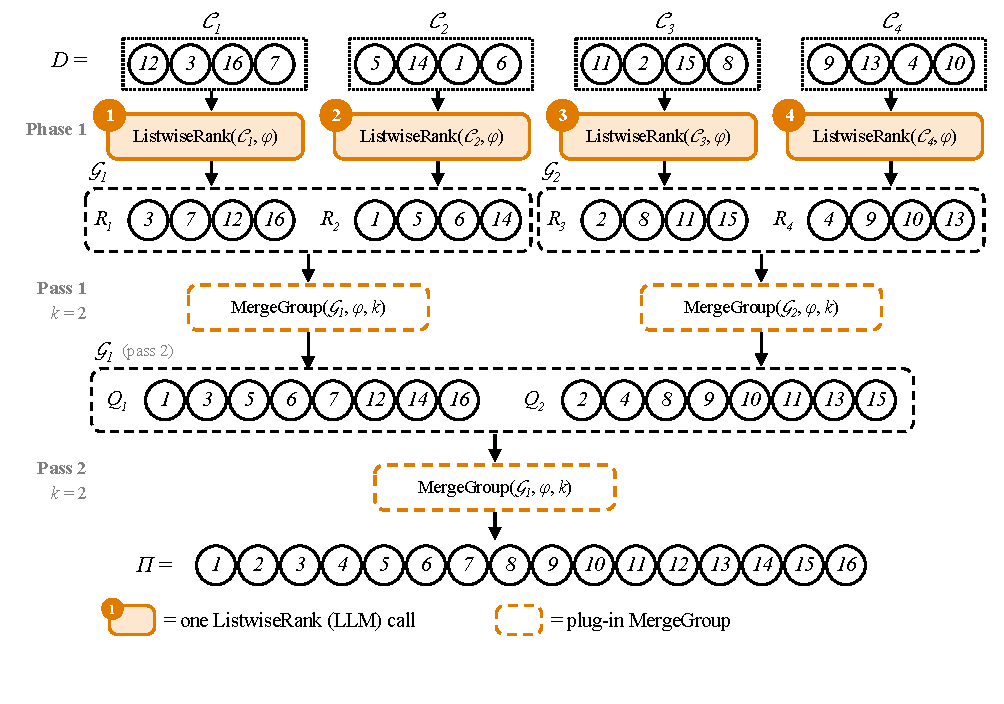
\includegraphics[width=0.95\linewidth]{fig/algo1-exp.pdf}
    \caption{Example of Algorithm~\ref{alg:semantic_external_merge}: 4 runs generation, then two merge passes.}
    \label{fig:exp:semantic_external_merge}
\end{figure}

\begin{example}\label{ex:alg1}
Fig~\ref{fig:exp:semantic_external_merge} traces Algorithm~\ref{alg:semantic_external_merge} on $n=16$ items with batch size $m=4$.
Phase~1 partitions $D$ into $r=\lceil 16/4\rceil=4$ chunks and sorts
each chunk with one listwise call, yielding 4 runs
$R_1$, $R_2$,
$R_3$, and $R_4$
(line~1--6). Phase~2 starts from $|\mathcal{L}|=4$; Suppose
\textsc{MergeCostModel} selects fan-in $k=2$ (line 7), therefore the sorting takes $\lceil\log_2 4\rceil=2$ merge passes. 
Pass~1
partitions $\mathcal{L}$ into $s=2$ groups,
$\mathcal{G}_1=\{R_1,R_2\}$ and $\mathcal{G}_2=\{R_3,R_4\}$, and merges
the groups in parallel through the \textsc{MergeGroup},
producing $Q_1$ and
$Q_2$ (lines~11--15). Pass~2 finally merges
$\{Q_1,Q_2\}$ into $\Pi=[1,\dots,16]$.
\end{example}



% \begin{example}\label{ex:alg1}
% Fig~\ref{fig:exp:semantic_external_merge} traces Algorithm~\ref{alg:semantic_external_merge} on $n=16$ items with batch size $m=4$.
% Phase~1 partitions $D$ into $r=\lceil 16/4\rceil=4$ chunks and sorts
% each chunk with one listwise call, yielding 4 runs
% $R_1=\langle 3,7,12,16\rangle$, $R_2=\langle 1,5,9,14\rangle$,
% $R_3=\langle 2,8,11,15\rangle$, and $R_4=\langle 4,6,10,13\rangle$
% (lines~3--6). Phase~2 starts from $|\mathcal{L}|=4$;
% \textsc{MergeCostModel} selects fan-in $k=2$ (line~9). Pass~1
% partitions $\mathcal{L}$ into $s=2$ groups,
% $\mathcal{G}_1=\{R_1,R_2\}$ and $\mathcal{G}_2=\{R_3,R_4\}$, and merges
% the groups in parallel through the plug-in \textsc{MergeGroup},
% producing $Q_1=\langle 1,3,5,7,9,12,14,16\rangle$ and
% $Q_2=\langle 2,4,6,8,10,11,13,15\rangle$ (lines~11--15). Pass~2 merges
% $\{Q_1,Q_2\}$ into $\Pi=\langle 1,\dots,16\rangle$, and line~16 strips
% the temporary identifiers. The schedule takes
% $\lceil\log_2 4\rceil=2$ passes; each numbered circle in the figure is
% one listwise call, and each dashed box is one \textsc{MergeGroup} algorithm 
% instance.
% \end{example}

\section{Sliding Window Multi-way Merge}
\label{sec:sw}

We propose a sliding window $k$-way merge algorithm as an instantiation of $\textsc{MergeGroup}$. The algorithm is an adaptation to listwise ranking from classical external $k$-way merge sort~\cite{DBLP:journals/csur/Graefe06}. 
In classical external $k$-way merge, the algorithm iteratively compares the current heads of the input runs and emits the smallest one. The ordering of the input runs is sufficient to guarantee that the emitted item is globally next.
For semantic \textsf{ORDER BY}, considering $\textsc{ListwiseRank}$ is the only available comparison primitive with a nontrivial cost, a direct head-by-head adaptation would therefore require one LLM call per emitted item.
To improve the throughput of $\textsc{ListwiseRank}$ regarding item emission, Algorithm~\ref{alg:sliding_window_kway_group_merge} packs head items from \emph{each} active run, so that a single call ranks up to $m$ candidate items across the group. In one $\textsc{ListwiseRank}$ call, since the LLM ranker can see only head items of the runs, its complete ranking output may not be globally ordered. The algorithm identifies a `safe prefix' from the output (line~18--22), and only emits this prefix. 



% Algorithm~2 merges a group of $k$ sorted runs by repeatedly ranking a
% window drawn evenly from all runs and emitting only the prefix of the
% ranking that can be certified as globally correct.

% The algorithm is the listwise counterpart of the $k$-way merge step of
% classical external merge sort~\cite{DBLP:journals/csur/Graefe06}. The
% classical merger repeatedly emits the smallest current run head: every
% decision is one exact two-item comparison, essentially free on a CPU,
% and the sortedness of the runs alone certifies each emission. Under a
% semantic order the only comparison primitive is a listwise call that
% ranks up to $m$ items at a fixed per-call price, so a head-by-head
% port would spend one call per emitted item. Algorithm~2 adapts the
% merge to this primitive: it packs items from \emph{all} active runs
% into one call, so a single call settles the relative order of up to
% $m$ items drawn across the group, and the certified-prefix rule
% (lines~18--22) restores the correctness argument that sortedness no
% longer provides, since the ranker sees only a bounded window of each
% run. The design also departs from the two-way external merge of prior
% LLM-based sorting~\cite{DBLP:journals/corr/abs-2509-00303}, which is
% in effect the $k=2$ instance of this scheme: hard-wiring the fan-in to
% two commits every schedule to $\lceil\log_2 r\rceil$ passes over $r$
% Phase-1 runs---the maximum over all feasible fan-ins---with every pass
% re-ranking the entire input. Algorithm~2 instead keeps the fan-in a
% free parameter, sound for any $g \ge 2$, and defers its choice to the
% cost model of \cref{sec:sw-cost}.

Algorithm~\ref{alg:sliding_window_kway_group_merge} maintains a read cursor $p_i$ for each run and an output sequence $\Pi$ (line 1). Each round of the loop (lines~3--24) issues one listwise call and emits a safe prefix of the LLM output. At the start of a round, line 3 identifies the active runs 
$A$, namely those with unread items.  If no active runs remain, the merge is complete (lines 4-5). If only one run remains active, lines 6–9 append its unread suffix directly to $\Pi$ without an LLM call, because it is already sorted. 
When more than one run remains active, line 10 divides the prompt budget evenly across them. Each active run receives a quota of $h=\lfloor m/|A| \rfloor$ items to be sorted by a $\textsc{ListwiseRank}$ call. 
Lines 11–16 assemble the batch $B$, where each active run $R_i$ contributes its next $b_i \leq h $ unread items, denoted as $W_i$. 
The algorithm also initializes a counter $e_i$  for each active run (line 15), recording how many contributed items from that run are emitted in the current round.
Line 17 invokes $\textsc{ListwiseRank}(B,\phi)$, producing a ranked order $\mathcal{O}$ over the batch. 
Lines~18--22 emit only the safe prefix of $\mathcal{O}$. The algorithm scans $\mathcal{O}$ in rank order,  appending each item to $\Pi$ and increasing the emitted counter $e_i$ of its  originating run. The scan stops once some run $R_t$ has had its contributed window fully emitted ($e_t=b_t$, lines~21--22).
This stopping criterion for emitting is required to ensure global orderedness: 
Once $W_t$ emits, the next unseen item from $R_t$ is not included in the current LLM call; it may therefore precede every remaining item in $\mathcal{O}$ under the semantic instruction $\phi$. Consequently, no item ranked after this point is safe as the next global output. 
Lines 23–24 then advance each cursor $p_i$ by exactly $e_i$ items emitted from that run. Any un-emitted suffix of $\mathcal{O}$ is processed again in the next call, where it competes against new arrival items from active runs. When all runs have been consumed, line 25 returns the merged sequence.

This algorithm is a generalization of the two-way external merge for LLM-based sorting~\cite{DBLP:journals/corr/abs-2509-00303}, which corresponds to the special case $k=2$. Fixing $k=2$ forces the merge schedule to use $\lceil\log_2 r\rceil$ passes over $r$ runs from Phase 1 of Algorithm~\ref{alg:semantic_external_merge}. 
In contrast, Algorithm~\ref{alg:sliding_window_kway_group_merge} emits $h$ items in the worst case, and $(h-1)|A|+1 \leq m-|A|+1$ in the best case. 
There exists an optimal fan-in $k$ in $\{2,\ldots, \lfloor m/2\rfloor\}$ maximizing expected item throughput of listwise calls (\cref{sec:cost}), where the upper bound ensures that each active run contributes at least two items and each listwise possibly emits more than one item. 

%, where the upper bound ensures that each active run contributes at least two items to a full window.

% Line~1 initializes a read cursor $p_i$ for every run and an empty
% output $\Pi$. Each iteration of the loop (lines~2--24) issues exactly
% one listwise call. Line~3 computes the set $A$ of active runs, those
% with unread items; lines~4--5 terminate when all runs are exhausted.
% Lines~6--9 handle the single-run case without any LLM call: when only
% one run remains active, its unread suffix is already sorted under
% $\phi$, because it was produced either by a Phase-1 listwise sort or
% by an earlier certified merge, so it is appended to $\Pi$ verbatim.

% Line~10 divides the window budget evenly among the active runs,
% giving each a quota of $h=\lfloor m/|A| \rfloor$ items so that the
% combined batch never exceeds the prompt capacity $m$. Lines~11--16
% assemble the batch $B$: every active run $i$ contributes the next up
% to $h$ unread items $W_i$ (fewer if the run is nearly exhausted); the
% counter $b_i$ records how many items run $i$ contributed and $e_i$
% counts how many of them are emitted in this round. Line~17 ranks the
% batch with one listwise call, yielding the order $\mathcal{O}$.

% Lines~18--22 emit the certified prefix of $\mathcal{O}$. The loop
% scans $\mathcal{O}$ in rank order, appends each item to $\Pi$, and
% credits its originating run; it stops as soon as some run $t$ has had
% its entire window emitted ($e_t=b_t$, lines~21--22). The stop is
% required for correctness rather than efficiency: once run $t$'s
% window is drained, the next unseen item of run $t$ may precede, under
% $\phi$, every remaining item in the batch, so no item ranked after
% this point can be certified as the global successor. Lines~23--24
% advance each cursor by exactly the emitted count $e_i$; the unemitted
% suffix of every window stays in place and re-enters the next batch,
% where it competes against fresh items from the previously exhausted
% run. Line~25 returns the merged run.

% Per listwise call, the emitted count therefore lies between $h$
% (worst case: the batch drains one window before emitting anything
% else) and $(h-1)|A|+1 = m-|A|+1$ (best case: every window retains one
% item when the first exhaustion occurs). 



\begin{algorithm}[t]
\small
\caption{Sliding-Window Semantic $k$-Way Merge}
\label{alg:sliding_window_kway_group_merge}
\KwIn{a group of sorted runs $\mathcal{G}=\{R_1,\dots,R_k\}$, instruction $\phi$, listwise batch size $m$}
\KwOut{one merged sorted run $\Pi$}

Initialize cursor $p_i \gets 0$ for every run $R_i$, $\Pi \gets [\ ]$ \;

\While{at least one run in $\mathcal{G}$ is not exhausted}{
    $A \gets \{R_i \mid p_i < |R_i|\}$ ; \algocomment{collect active runs} \\
    \If{$A=\emptyset$}{
        \textbf{break} \;
    }
    \If{$|A|=1$}{
        let $R_u$ be the only active run in $A$ \;
        Append $R_u[p_u:|R_u|]$ to $\Pi$ \;
        \textbf{break} \;
    }

    $h \gets \lfloor m / |A| \rfloor$ ; \algocomment{window size contributed by each active run} \\
    $B \gets [\ ]$ \;

    \ForEach{$R_i \in A$}{
        $W_i \gets$ up to $h$ items from $R_i[p_i:]$ \;
        $b_i \gets |W_i|$ ; \algocomment{items contributed by run $i$ in this batch} \\
        $e_i \gets 0$ ; \algocomment{items emitted from run $i$ in this batch} \\
        Append $W_i$ to $B$ \;
    }

    $\mathcal{O} \gets \textsc{ListwiseRank}(B,\phi)$ \;

    \ForEach{$x \in \mathcal{O}$}{
        let $R_t$ be the originating run of $x$ \;
        Append $x$ to $\Pi$, $e_t \gets e_t + 1$ \;
        \If{$e_t = b_t$ \textbf{and} $p_t + b_t < |R_t|$}{
            \textbf{break} ; \algocomment{run $R_t$ drained its window but still has unseen items} \\
        }
    }

\ForEach{$R_i \in A$}{
    $p_i \gets p_i + e_i$ ; \algocomment{update cursors; unsafe suffix of $\mathcal{O}$ stay pending} \;
}
}

\Return{$\Pi$}
\end{algorithm}

% Approved: PR9 cursor/sw-sliding-window-figure-ad37, recovery/sw/sw-wide.pdf
\begin{figure*}[t]
    \centering
    \includegraphics[width=\textwidth]{sw-wide.pdf}
    \caption{Example of Algorithm~\ref{alg:sliding_window_kway_group_merge} for sliding window merge $(m = 8, h = \lfloor m / |A|\rfloor)$: three calls emit $5+5+6=16$ items.
    \emph{Integration note:} synthetic layout placeholder for type-setting review; not a measured execution trace.}
    \label{fig:eg:sliding_window}
\end{figure*}

\begin{example}\label{ex:alg2}
Fig.~\ref{fig:eg:sliding_window} illustrates a sliding-window merge with $k = 4$ sorted runs and batch size $m = 8$. In Round 1, all runs are active, so each receives quota $h=\lfloor 8/4\rfloor=2$. The batch contains the first two unread items from each run, $B=\{3,7,1,5,2,8,4,9\}$. The listwise call returns $\mathcal{O} = [1, 2, 3, 4, 5, 7, 8, 9]$. The algorithm emits the safe prefix $[1, 2, 3, 4, 5]$ and stops when $R_2$'s window $[1, 5]$ is exhausted, because the unseen item $6$ from $R_2$ may precede the remaining ranked items. 
In Round 2, the unemitted items ${7, 8, 9}$ re-enter the batch together with new arrival items, forming a batch $B = \{7,12,6,14,8,11,9,10\}$. The The listwise call returns $\mathcal{O} = [6,7,8,9,10,11,12,14]$. The safe prefix $[6, 7, 8, 9, 10]$ is emitted and the scan stops $R_4$'s window $[9, 10]$ is exhausted. The process continues until full ranking $\Pi$ is generated over $k$ runs. 

% Algorithm~2 on the four Phase-1 runs of Figure~1 with
% $m=8$. In Round~1 all four runs are active, so each receives a quota
% $h=\lfloor 8/4\rfloor=2$ and contributes its next two items, giving
% $B=\{3,7,1,5,2,8,4,6\}$; one listwise call returns
% $\mathcal{O}=\langle 1,\dots,8\rangle$. The emission loop appends
% $1,2,3,4,5$ and then stops: run $R_2$ has had its entire window
% emitted ($e_2=b_2=2$) while it still holds unseen items, and the
% unseen item $9$ may precede $6,7,8$ under $\phi$, so $6,7,8$ cannot be
% certified and re-enter the next batch (lines~21--22). Round~2
% assembles $B=\{7,12,9,14,8,11,6,10\}$ and emits $6,\dots,10$, again
% truncated after five items when $R_4$'s window drains. In Round~3 the
% nearly exhausted runs contribute $b_2=b_4=1$, so $|B|=6$; every
% draining run is fully exhausted, no truncation applies, and all six
% items $11,\dots,16$ are emitted. Three calls emit $5+5+6=16$ items,
% between the per-call bounds $h$ and $m-|A|+1$ of Section~4.
\end{example}

\section{Loser Tree Multi-way Merge}
\label{sec:lt}

This section proposes algorithmic instantiations of $\textsc{MergeGroup}$ via tournament data structures, including two algorithms with a loser tree~(\cref{sec:lt:binary}) and an optimized segmented loser tree (\cref{sec:lt:segment}). 

\subsection{Loser Tree}
\label{sec:lt:binary}

Algorithm~\ref{alg:loser_tree_kway_group_merge} replaces the flat window of Algorithm~\ref{alg:sliding_window_kway_group_merge} 
with a loser tree over $k$ runs. 
Recall the classical loser tree used in external merge sort~\cite{DBLP:journals/csur/Graefe06}; the leaves correspond to the $k$ runs, and each internal node stores the loser of a match between two subtree winners, and the root stores the overall champion. 
When a leaf is updated, only the $O(\log k)$ matches on the path to the root should be recomputed. This order locality makes loser tree suitable for tournament-style LLM ranking. 
Algorithm~\ref{alg:loser_tree_kway_group_merge} adapts classical loser tree to listwise LLM ranking at two points. First, a loser tree is initialized by \textsc{InitLoserTree}, ranking $k$ run heads in a single listwise call. Second, leaf update triggers a \textsc{RefreshPath}, batching the updated run head together with the stored losers along the affected path and ranking this set in one listwise call.



% structure. A loser tree over $k$ runs maintains, after $O(\log k)$
% comparisons per update, the invariant that the root's current winner
% is the globally best unemitted item; a merge then reduces to
% repeatedly popping the root and repairing a single leaf-to-root path.


% The loser tree is the classical tournament structure of external merge
% sort~\cite{DBLP:journals/csur/Graefe06}: leaves hold the $k$
% contestants, each internal node remembers the loser of one match, the
% root holds the champion, and replacing a leaf re-plays only the
% matches on that leaf's bracket path, since every other recorded
% outcome is unaffected. Exactly this match locality makes the structure
% relevant to tournament-style LLM
% ranking~\cite{DBLP:journals/corr/abs-2603-17223}, in which the model
% acts as the judge of each match: the matches invalidated by one
% emission form a single short path, a closed candidate set of at most
% $1+\lceil\log_2 g\rceil$ items that fits comfortably into one prompt.
% The classical merger, however, plays the path as a chain of exact
% pairwise comparisons---free on a CPU, but one LLM call each under a
% semantic order, and inherently sequential because every match waits
% for the winner of the previous one. Algorithm~3 adapts the structure
% to the listwise primitive at both interaction points:
% \textsc{InitLoserTree} ranks the $k$ run heads in one call and replays
% the entire construction tournament through rank-map lookups in place
% of $g-1$ comparison calls, and \textsc{RefreshPath} batches the new
% representative together with the stored losers of the path into one
% listwise call whose local ranks settle all path matches at once. The
% tournament bookkeeping is inherited verbatim; only the comparison
% currency changes, and the price of a pop drops from
% $\lceil\log_2 g\rceil$ sequential decisions to exactly one call.

We explain the detailed procedure of Algorithm~\ref{alg:loser_tree_kway_group_merge}. Line 1 initializes the read cursors $p_i$, and line 2 forms the set of active runs $A$. 
Lines 3–4 handle the degenerate case in which all runs are empty. Lines 5–6 collect the head item of each active run, i.e., its current representative $x_i$. In line 7, the algorithm initializes the loser tree by $\textsc{InitLoserTree}$, and the output permutation $\Pi$. The main loop in lines 8–19 emits one item per round, triggering one listwise call in the procedure $\textsc{RefreshPath}$ for tree maintenance (line 19). 
Lines~9--12 address the corner case in which a single active run remains, similar to lines 6--9 in Algorithm~\ref{alg:sliding_window_kway_group_merge}. 
The algorithm pops the current winner $x_u$ from the root, which originally comes from run $R_u$ (line 13). Based on the order locality of loser tree, $x_u$ is the current highest-ranked representative and the next global output item. Line 14 therefore emits $x_u$ to $\Pi$ and advances the cursor of $R_u$. Lines 15-16 extract the new head item from $R_u$ as the new representative $x_u$ if $R_u$ is non-exhausted; otherwise, $R_u$ is deactivated (lines 17--18).
Finally, line 19 calls $\textsc{RefreshPath}$ to maintain the locality of the loser tree, which spends exactly one listwise call. We first briefly introduce the path refresh algorithm, $\textsc{RefreshPath}$, followed by tree construction, $\textsc{InitLoserTree}$.
 
% Line~1 initializes the cursors, and line~2 restricts attention to the
% set $A$ of non-empty runs; lines~3--4 dispose of the degenerate empty
% input. Lines~5--6 load the head of every active run as its current
% representative $X_i$. Line~7 builds the loser tree with
% $\textsc{InitLoserTree}$ (Algorithm~\ref{alg:init_loser_tree}) and initializes the output.

% The main loop (lines~8--19) emits one item per iteration.
% Lines~9--12 are the single-run fast path of Algorithm~2: the last
% surviving run's suffix is appended without further LLM calls.
% Line~13 reads the overall winner $u$ at the root, whose
% representative $X_u$ is the highest-ranked unemitted item under
% $\phi$. Line~14 emits $X_u$ and advances run $u$'s cursor.
% Lines~15--18 either promote run $u$'s next item to be its new
% representative or, if run $u$ is exhausted, remove $u$ from $A$ and
% deactivate its leaf. Line~19 restores the tree invariant with
% $\textsc{RefreshPath}$ (Algorithm~\ref{alg:refresh_loser_tree_path}). Only the nodes on the path from
% $\text{Leaf}(u)$ to the root can be affected by the change at leaf
% $u$, so each emission touches at most
% $\lceil \log_2 g \rceil$ internal nodes and, as shown below, costs
% exactly one listwise call.
\stitle{Tree construction:} 
$\textsc{InitLoserTree}$ constructs the initial loser tree over the representatives of the $k$ runs, at most, in one group. 
Listwise ranking computes the ranking of the $k$ representatives and returns a rank map $\rho$ for lookup. If $k \leq m$, one listwise call can accommodate these representatives; Otherwise, if $k > m$, we invoke two-way sliding window merge to process the ranking. Then, $\textsc{InitLoserTree}$ initializes a complete binary tree, padding empty leaves with \textsc{null} and replays the tournament bottom-up by looking up $\rho$ for pairwise item comparison. When both children are non-null, the child with the higher rank wins and  propagates upward. After all matches are replayed, the root stores the global winner of the current group. 


% e$\textsc{InitLoserTree}$ (Algorithm~\ref{alg:init_loser_tree}) constructs an initial loser tree over the representatives of the $g$ runs in the current group. Unlike classical tournament tree construction, which performs a pairwise comparison at every internal node, listwise ranking first obtains a global order over all resident candidates and then builds the loser tree  through rank-map lookups, avoiding an LLM call for each match. 

% Specifically, $\textsc{InitLoserTree}$ collects the $X_{\mathrm{init}}=\{x_i\mid i\in A\}$ resident representatives. If $|X_{\mathrm{init}}|\le m$, one listwise call ranks them. Otherwise, it ranks batches of at most $m$ items and repeatedly merges the two shortest resulting runs with the fan-in-two sliding-window merger. The final run $Q_{\mathrm{init}}$ defines the rank map $\rho$.

% The algorithm then seeds a complete binary loser tree, pads unused leaves with \textsc{null}, and replays the tournament bottom-up using $\rho$. A \textsc{null} child forwards the other candidate; otherwise, the winner propagates upward and the loser is stored at the node. The root stores the resulting global winner.

%Line~1 ranks these representatives with one listwise call, and 
%line~2 converts the returned order into a rank map $\rho$ as an index for subsequent lookup. 
%Line 3 allocates a complete binary tree, padding the empty leaves with \textsc{null}, and lines 3-7 seed the leaves with the representatives. Lines 8–18 then play the tournament bottom-up, where pairwise comparisons look up the index $\rho$. After construction, the root gives the current global winner in $O(1)$ time. 

% Line~1 ranks the $k$ representatives with a single listwise call, and
% line~2 converts the returned order into a rank map $\rho$. All
% comparisons during construction are then $\rho$-lookups, so building
% the tree issues no further LLM calls. Line~3 allocates a complete
% binary tree, padding the leaf level to a power of two with
% \textsf{null} leaves; lines~4--7 seed the leaf winners. Lines~8--18
% play the tournament bottom-up: at every internal node the two child
% winners are compared through $\rho$ (lines~15--18), the winner
% propagates upward, and the loser is stored at the node;
% \textsf{null} children simply forward the other child (lines~11--14).
% The resulting structure supports winner extraction in $O(1)$ and path refresh in $O(\log k)$.

% In steady state the merger thus pays one listwise call over
% $O(\log k)$ items per emitted element. \cref{sec:slt} introduces a segmented variant in which each leaf holds a segment of $h$ items and each refresh emits $h$ items per call; \cref{sec:lt-cost} models the call count of both variants and derives the optimal fan-in for each.
\stitle{Path refresh:}
$\textsc{RefreshPath}$ maintains loser tree orderedness after one representative of run $R_u$ updates. Unlike the maintenance of a classical loser tree, which scans the affected path once, path refresh with a listwise ranking sweeps the affected path twice: the first sweep collects the items to be ranked in one batch, and the second pass updates the path using the ranking output. 
Specifically, $\textsc{RefreshPath}$ first collects the batch $B$ to be ranked. This set contains the updated representative of run $R_u$ if $R_u$ is still active, together with the stored losers on the path from $\text{Leaf}(R_u)$ to the root. Losers belonging to exhausted runs are skipped. Since the path contains at most one stored loser per level, $|B| \le 1+\lceil \log_2 k \rceil$. Then, items in $B$ are sorted by a listwise call, and a rank map $\rho_{path}$ preserves the ranking.
The second sweep replays the standard tournament along the same path, where pairwise comparisons look up the index $\rho_{path}$.
%A variable $w$ stores the candidate currently propagating upward, initialized to the updated run $R_u$ or to \textsc{null} if $R_u$ has been exhausted (lines 16--19). In lines 20--33, along each ancestor node, $w$ is compared with the node’s stored loser $r$ using path $\rho_{path}$. The higher-ranked candidate continues upward, and the lower-ranked one becomes the node’s new stored loser. If either side is null because a run has been exhausted, the non-null candidate is forwarded. 
When the replay reaches the root, all affected matches have been repaired, and $\textsc{CurrentWinner}(T)$ will return the next global best.

% The procedure runs in two sweeps over the same path. The first sweep
% (lines~1--10) collects the comparison set $\mathcal{P}$: the updated leaf's new
% representative, if run $u$ is still active (lines~2--3), together
% with the stored losers along the path from $\text{Leaf}(u)$ to the
% root (lines~5--10), skipping losers whose runs are exhausted. Since
% the path holds one stored loser per level,
% $|P| \le 1+\lceil \log_2 g \rceil$. Lines~11--12 short-circuit when
% there is nothing to compare. Line~13 ranks $P$ with a single listwise call and line~14 builds the local rank map $\rho_{path}$; this is the only LLM interaction of the refresh. The second sweep (lines~15--33)
% replays the tournament along the path: $a$ holds the candidate
% propagating upward, initialized to $u$ or \textsf{null}
% (lines~16--19). At every ancestor, the candidate meets the stored
% loser $q$; the one ranked higher by $\rho_{path}$ continues upward
% while the other is stored as the node's new loser (lines~28--32), and
% the \textsf{null} cases arising from exhausted runs are resolved by
% forwarding whichever side remains (lines~23--27). When the sweep
% reaches the root, the invariant holds again and
% $\textsc{CurrentWinner}(T)$ is the next global head.

The loser tree maintains global orderedness for the current representatives of all active runs. This design is distinguished from a tournament graph-based LLM ranking in the ListK framework~\cite{DBLP:journals/corr/abs-2603-17223}. In this tournament LLM ranking, there is no explicit data structure to maintain global orderedness; therefore, the algorithm is brittle to possible inconsistent results across different listwise calls. 
The loser tree merge sort emits one item after a listwise call (in $\textsc{RefreshPath}$).
To improve the item throughput regarding listwise calls, \cref{sec:lt:segment} introduces a segmented variant in which each leaf holds a segment of $h$ items, and each refresh emits $h$ items per call.




\begin{algorithm}[t]
\small
\caption{Loser-Tree Semantic $k$-Way Merge}
\label{alg:loser_tree_kway_group_merge}
\KwIn{a group of sorted runs $\mathcal{G}=\{R_1,\dots,R_k\}$, instruction $\phi$}
\KwOut{one merged sorted run $\Pi$}

Initialize cursor $p_i \gets 0$ for every run $R_i$ \;
$A \gets \{R_i \mid |R_i|>0\}$ ; \algocomment{indices of non-empty runs} \\
\If{$A=\emptyset$}{
    \Return{$[\ ]$} \;
}

\ForEach{$R_i \in A$}{
    $x_i \gets R_i[p_i]$ ; \algocomment{current representative of run $i$} \\
}

$T \gets \textsc{InitLoserTree}(A,\{x_i \mid R_i\in A\},\phi)$, $\Pi \gets [\ ]$ \;

\While{$A \neq \emptyset$}{
    \If{$|A|=1$}{
        let $R_u$ be the only active run in $A$ \;
        Append $R_u[p_u:|R_u|]$ to $\Pi$ \;
        \textbf{break} \;
    }

    $R_u \gets \textsc{CurrentWinner}(T)$ \;
    Append $x_u$ to $\Pi$, $p_u \gets p_u + 1$ \;

    \eIf{$p_u < |R_u|$}{
        $x_u \gets R_u[p_u]$ \;
    }{
        Remove $R_u$ from $A$ and mark $\textsc{Leaf}(R_u)$ inactive in $T$ \;
    }

    $T \gets \textsc{RefreshPath}(T,R_u,A,\{x_i \mid R_i\in A\},\phi)$ \;
}

\Return{$\Pi$} \;
\end{algorithm}




% Approved: PR3 cursor/lt-h-main-figure-d022, recovery/lt/lt-h-main.pdf
\begin{figure*}[t]
  \centering
  \includegraphics[width=\textwidth]{lt-h-main.pdf}
  \caption{Pointer-guided LT($h$) on the shared 16-element runs
  ($k{=}4$, $h{=}2$).
  Gray lines are tree edges.
  A black curve is the child pointer; on the refresh it runs beside the
  straight refresh path, not on it.
  The blue arrow is a separate winner exit: the pair drawn in the root box
  is the stored loser and is not the value the arrow carries.
  (a)~After initialization the winner $[1,2]$ has already left.
  (b)~Call~1 input is $[3,4,5,6,7,14]$, the red-bordered segments.
  The right subtree is not in that call.
  (c)~The winner exit is $[3,4]$.
  The root and the left node keep the losers returned by call~1.
  $h{=}1$ is the same generator with a shorter segment.
  \emph{Integration note:} synthetic layout placeholder for type-setting review.}
  \label{fig:eg:loser_tree_kway_group_merge}
\end{figure*}
% Approved: PR6 cursor/pointer-local-figure-1615 scheme A
\begin{figure}[t]
  \centering
  \includegraphics[width=\linewidth]{pointer-scheme-a.pdf}
  \caption{Local pointer rule on one internal node ($h=2$).
    Child 0 is run $R_1$ and child 1 is run $R_2$.
    Slot 0 and slot 1 are replay arguments, not child names.
    Build assigns pointer $=$ child 1.
    The next refresh follows that child.
    Refresh returns pointer $=$ child 0; the previous value was child 1.
    A returned pointer may name the same child.
    That case is not in the trace and is not drawn.
    \emph{Integration note:} synthetic layout placeholder for type-setting review.}
  \label{fig:eg:pointer-rule}
\end{figure}

% ---------------------------------------------------------------------
% Example 3  (place near Figure 3, end of Section 5.1)
% ---------------------------------------------------------------------
\begin{example}\label{ex:alg3}
Fig.~\ref{fig:eg:loser_tree_kway_group_merge} illustrates Algorithm~\ref{alg:loser_tree_kway_group_merge} on the same $k=4$ sorted runs to Example~\ref{ex:alg2}, i.e., $R_1$, $R_2$, $R_3$ and $R_4$.
In Fig.~\ref{fig:eg:loser_tree_kway_group_merge}(a), \textsc{InitLoserTree} collects the four run heads $\{3,1,2,4\}$ and ranks them with one listwise call, obtaining the order $[1, 2, 3, 4]$. This order is used to construct the initial loser tree without further LLM calls. The root winner is therefore item 1, which is emitted first. Run $R_2$ then advances, and its new representative becomes 5. 
Fig.~\ref{fig:eg:loser_tree_kway_group_merge}(b) shows performing \textsc{RefreshPath} on the leaf $R_2$. Only the path from the leaf of $R_2$ to the root may have changed. The algorithm collects the new representative 5 together with the stored competitors on this path, forming a batch $B = \{ 2, 3, 5 \}$, A single listwise call returns $ [2, 3, 5 ]$, which simultaneously resolves all comparisons on the path. The refreshed root winner is item 2, so that 2 is emitted and $R_3$ advances to representative item $8$.
Fig.~\ref{fig:eg:loser_tree_kway_group_merge}(c) refreshes the path from $R_3$. Similarly, a listwise call ranks batch $B = \{3, 4, 8\}$ and item $3$ becomes the next root winner. In this example, each emit only affects one path and requires one listwise ranking over at most $1+\lceil\log_2 4\rceil=3$ items. 

% \textsc{InitLoserTree} ranks the four run heads $\{3,1,2,4\}$ with a
% single listwise call and converts the result into the rank map
% $\rho$; the tournament is then built by $\rho$-lookups alone, storing
% one loser per internal node ($3$ and $4$ at the lower level, $2$ at
% the root) and propagating $R_2$'s head to the root. Pop~1 emits $1$.
% \textsc{RefreshPath}$(R_2)$ collects the comparison set
% $P=\{5,3,2\}$, the new representative of $R_2$ plus the stored losers
% on its leaf-to-root path, with $|P|\le 1+\lceil\log_2 4\rceil=3$. One
% listwise call ranks $P$; the second sweep replays the tournament
% along the path, storing $5$ and $3$ as new losers, and pop~2 emits
% $2$ from $R_3$. \textsc{RefreshPath}$(R_3)$ analogously ranks
% $P=\{8,4,3\}$, and pop~3 emits $3$ from $R_1$. Each emission thus
% costs exactly one listwise call over at most three items, and only
% the highlighted path nodes are touched; the rest of the tree is
% untouched.
\end{example}




\subsection{Segmented Loser Tree}
\label{sec:lt:segment}

Recall that Algorithm~\ref{alg:loser_tree_kway_group_merge} emits exactly one item per path refresh that spends one listwise call, and each listwise call ranks $O(\log_2 k)$ items on a path from leaf to root. This number of items to rank is commonly smaller than the actual batch size $m$ of a listwise call, which is in about $[10, 30]$, depending on the effective context length and the expectation of the item tokens. This under-utilization of listwise calls degrades the throughput of item emission, which motivates us to design an optimized structure to maintain the global orderedness for more items. Segmented loser tree extends a binary loser tree by accommodating a segment of $h$ items in one node instead of a single representative. The root also stores the $h$ winners, which emit together after path refreshing via one listwise call. With the gist of the $k$-way merge algorithm (Algorithm~\ref{alg:loser_tree_kway_group_merge}), \textsc{InitLoserTree} and \textsc{RefreshPath} unchanged, the differences from the segmented loser tree algorithm lie in three aspects as follows:


% The binary merger of
% Algorithm~\ref{alg:loser_tree_kway_group_merge} pays exactly one
% listwise call per emitted item: a pass over $n$ items issues $n$
% path-refresh calls, yet each call ranks only the $O(\log k)$
% representatives of one root path---a small fraction of the $m$ items
% a single prompt can hold. The segmented loser tree removes this
% throughput bottleneck by making every tree slot hold a
% \emph{segment} of items instead of a single representative, so that
% one ranking call moves $h$ items through the tree at once. The tree
% topology, the initialization discipline, and the leaf-to-root
% refresh of
% Algorithms~\ref{alg:loser_tree_kway_group_merge}--\ref{alg:refresh_loser_tree_path}
% carry over unchanged; the variant differs in three respects.

\etitle{Segments in tree nodes.} Each leaf stores up to $h$ consecutive unread items from its run. After passing a segment to its parent, an internal node retains at most $h$ items and records which child must be replenished before more items can pass. Let $d=\max(1,\lceil \log_2 k \rceil)$ be the maximum number of internal nodes on a leaf-to-root path. A path refresh contains one new leaf segment and at most one retained segment at each level, and hence ranks at most $(1+d)h$ items. We therefore choose $h=\lfloor m/(1+d) \rfloor$ so that one refresh fits in a listwise call.

%\etitle{Segments in tree nodes.} Each leaf stores up to $h$ consecutive unread items from its run, each internal node stores a loser segment of up to $h$ items, and the root stores $h$ winners. Let $d=\max(1,\lceil \log_2 k \rceil)$ be the maximum number of internal nodes in a path from leaves to root. Since a path refresh ranks the refreshed leaf segment together with the $d$ loser segments stored along that path, the batch size is at most $(1 + d)h$, and the accommodation in one listwise call requires $(1+d)\,h \le m$. We therefore choose $h=\lfloor m/(1+d) \rfloor$.


\etitle{Pointer-guided path refresh.} After emitting $h$ items, the overall path refresh is similar to the two-sweep procedure of the original loser tree. 
A sweep first collects $(1+d)h$ items to rank from a leaf-to-root path, and a second sweep ranks these items by a listwise call, replaying the tournament bottom-up and updating the losers of internal nodes and the winner in the root. The original loser tree can be regarded as a special case of $h = 1$.
It is worth noting that the main difference is the selection of an affected path, from the root to an active run that can supply $h$ new representatives, as there may be more than one run emitting their heads. Simultaneously, refreshing along this path should ensure the global orderedness of these items. We achieve this path identification and order maintenance by adding a `blocked-child' pointer in each internal node and the root of the tree.
Intuitively, for a node, this blocked-child pointer identifies either its left or right subtree, which will emit at least $h$ items earlier under two-way merge, following the ordering result from the listwise rank map. 
Therefore, pointers from the root to leaf identify the current `frontier' of the recursive two-way merge process presented as the segmented loser tree. 

After emitting $h$ items, the pointers identify the affected path, and the active run in the leaf node supplies $h$ items. The algorithm collects the items from $(1 + d)$ segments and performs one listwise call. Subsequently, tournament replay updates the $h$ losers for each internal node in a bottom-up fashion. During the replay, an ascending pool of $h$ items moves upward. At each level, this pool is merged with the $h$-item segment retained at that node by looking up the listwise rank map $\rho$, until the $h$-item winner reaches the root.  
More importantly, the algorithm updates the blocked-child pointer by referring to the ranking result in $\rho$. Through the pointers, the algorithm indirectly maintains the global order of all $h$-item segments in the tree.

% The algorithm then collects the new leaf segment and all retained segments on the leaf-to-root path, and ranks their union with one listwise call. To stabilize the listwise batch size, every node advances only complete $h$-item segments and retains an $h$-item segment for the next refresh, giving a fixed batch size of $(1+d)h \le m$. The returned local rank map is sufficient to replay all affected matches without further comparisons. During the replay, an ascending pool of $h$ items moves upward. At each level, this pool is merged with the $h$-item segment retained at that node. The next $h$ safe items continue upward, while the other $h$ items remain at the node; the child whose segment is exhausted first determines the blocked child for the next refresh. Thus, both the ascending pool and the retained segment remain of size $h$ throughout a full path, except at run tails. When the pool reaches the root, it forms the next output segment, which can be emitted without another ranking call. Consequently, a full refresh emits $h$ items at the cost of one listwise call.


%\etitle{Balanced-halving path refresh.} After emitting $h$ items, the algorithm refreshes a path by supplying $h$ new representatives from an active run. 
%{\color{red}As more than one run may emit their representatives, the algorithm breaks the tie by prioritizing the leaf in which the run is exhausted, followed by the leaf with the fewest items remaining in the tree.}
%A refresh first reloads the selected leaf with the next $h$ unread items from its run. It then collects this leaf segment and the loser segments on the leaf-to-root path, and ranks their union with one listwise call. The returned local rank map is sufficient to replay all affected matches, without any additional comparisons. During the replay, an ascending pool of up to $h$ items moves upward. At each level, this pool is merged with the stored loser segment at that node.  Among the resulting at most $2h$ items, the top $h$ items under $\phi$ continue upward, while the remaining items become the node’s new loser segment. Thus, the pool size remains $h$ throughout the path, except at final segments near exhaustion. When the pool reaches the root, it forms the next output segment and is appended to the tree’s output buffer, which can then be drained without further ranking calls. Consequently, a full refresh emits $h$ items at the cost of one listwise call. 
% improving over the binary variant’s one item per call.

% {\color{blue}When two child segments compete at an internal node, their merged output continues until one child segment is exhausted, while the other still contains remaining items. These remaining items cannot yet be passed upward: although their order relative to the exhausted segment is known, their order relative to the next segment from the sibling is not. The parent produces its output by consuming the items supplied by its two children. Once one child segment becomes empty, the parent is therefore blocked on that child and stops before draining the remaining sibling segment. To resume its output, the algorithm must replenish the exhausted child. Starting from the root and repeatedly selecting the blocked child determines a unique root-to-leaf path; the leaf of this path identifies the active run to refresh, without any tie-breaking among runs.}



\etitle{Segment initialization.}  The initialization stage ranks all $kh$ items resident in leaves, instead of only the $k$ run heads.  If all $k h$ items fit into one listwise call, i.e., $k h \leq m$, a single call suffices to obtain their global order; Otherwise, if the $k h$ items exceed the batch limit of one listwise call, $\textsc{InitLoserTree}$ applies a 2-way sliding window merge to produce a rank map over these items. 
The segmented loser tree is then constructed bottom-up with all the block-child pointers initialized using only rank map lookups.


% \stitle{Windowed initialization.}
% Before the first refresh, the global rank map must cover the
% $k h$ items initially resident in the leaf segments rather than the
% $k$ run heads. Following Algorithm~\ref{alg:init_loser_tree}, the
% items are first interleaved across runs in a round-robin fashion so
% that the run heads appear at the front of the sequence. If all $k h$
% items fit into one listwise batch, a single call yields their global
% order; otherwise the order is assembled by $\lceil k h/m \rceil$
% successive calls, each ranking a full batch of $m$ items, committing
% a prefix of the returned order, and carrying the remaining suffix
% into the next batch, so that consecutive batches are stitched into
% one total order. Tree construction then proceeds bottom-up using only
% the resulting rank map and remains free of LLM calls.


For both loser tree ($h = 1$) and segmented loser tree ($h > 1$), throughput gain comes with a trade-off. Since $h=\lfloor m/(1+d) \rfloor$, the listwise output per call decreases as the fan-in $k$ increases through $d = \lceil \log_2 k \rceil$, while the number of merge passes also declines. Consequently, the overall throughput of the merge tree is not necessarily monotonic in \(k\), as it is jointly determined by the per-call output and the number of merge passes.
As $d \geq 1$ implies $d \leq m - 1$, and hence $k \le 2^{m-1}$. There exists an optimal fan-in $k$ in $\{2,\ldots, 2^{m-1}\}$ minimizing the expected total number of listwise calls (\cref{sec:cost}).


% This throughput gain comes with a trade-off. Since $h=\lfloor m/(1+d) \rfloor$, the listwise output per call decreases as the fan-in $k$ increases through $d = \lceil \log_2 k \rceil$, while the number of merge passes also declines. Moreover, each refresh must fit the $1+d$ segments along a path into one listwise batch; {\color{red}requiring $d \geq 1$ implies $d \leq m - 1$, and hence $k \le 2^{m-1}$. This fan-in cap is absent in the original loser tree.} Thus, increasing $k$ reduces the number of merge passes but also decreases the number of items emitted per call.

% The throughput gain is not free: $h=\lfloor m/(1+d) \rfloor$ shrinks
% as the fan-in grows through $d$, and feasibility requires the $1+d$
% segments of a root path to fit into one batch, capping the fan-in at
% $k \le 2^{m-1}$---a constraint the binary variant does not have.
% Larger $k$ thus buys fewer merge passes but smaller per-call output;
% \cref{sec:lt-cost} quantifies both forces and selects the fan-in
% that minimizes the total call count.


\begin{figure}
    \centering
    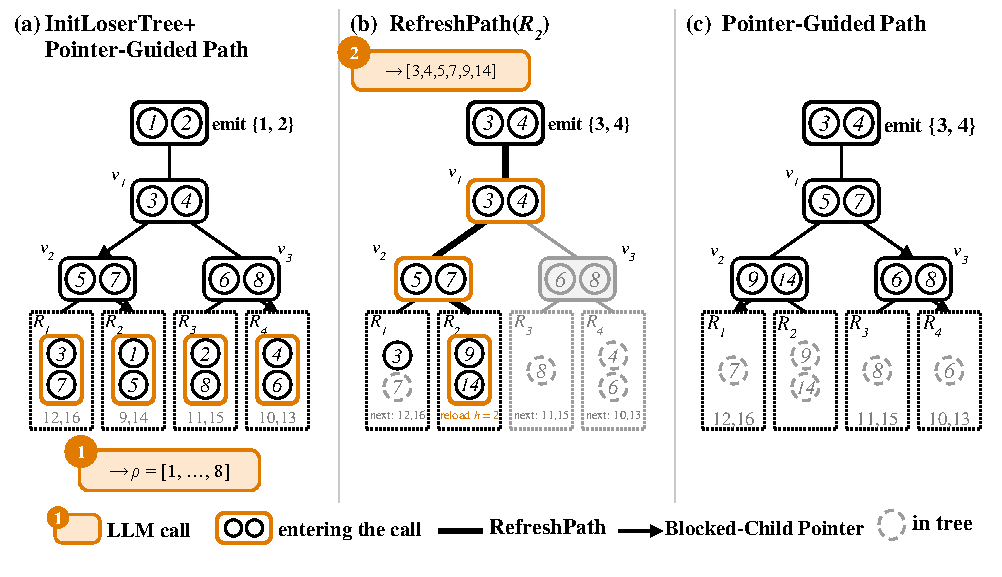
\includegraphics[width=0.95\linewidth]{fig/segment_loser_tree_exp.pdf}
    \caption{Segmented loser tree ($m  = 8 \Rightarrow d =2, h = 2$) }
    \label{fig:eg:segment_loser_tree}
\end{figure}

\begin{example}\label{ex:alg3seg}
Fig.~\ref{fig:eg:segment_loser_tree} illustrates a segmented loser tree with fan-in $k = 4$ and a listwise batch size $m = 8$. 
Thus, the tree depth $d=\max(1,\lceil\log_2 4\rceil)=2$ and the segment length $h=\lfloor 8/(1+2)\rfloor=2$. 
In Fig.~\ref{fig:eg:segment_loser_tree}(a), each leaf, $R_1$, $R_2$, $R_3$, and $R_4$, load two head items, 
These eight items are ranked by one listwise call, and the tree is initialized by bottom-up tournaments where two loser items are retained in each node. The blocked-child pointers identify when the winner $[1, 2]$ is emitted, either left or right subtree will be refreshed. For node $v_2$ with loser $[5, 7]$, a two-way merge of its children $R_1, R_2$ will first exhaust the items $[1,5]$ because of the local order $[1, 5, 3, 7]$. $R_1$ is non-exhausted due to 7 falling behind $5$. Therefore, the pointer of $v_2$ points to the leaf with $R_2$. Similarly, the internal node $v_1$ points its child $v_2$. That is because at node $v_1$, winner $[1, 3]$ from $v_2$ competes with winner $[2, 4]$ from $v_1$, and the merge result $[1, 2, 3, 4]$ making $v_2$ earlier exhausts its winner. From the perspective of two-way merge, the pointer identifies which child provide a safe prefix, and temporary blocks refreshing on the other child. 
After the winner $[1, 2]$ emits, the affect path $(v_1, v_2, R_2)$ is identified. Two items are refilled into $R_2$ and a listwise call is used to refresh this path as shown in Fig.~\ref{fig:eg:segment_loser_tree}(b). 

% In Fig.~\ref{fig:eg:segment_loser_tree}(a), the four initial leaf segments $R_1$, $R_2$, $R_3$, and $R_4$ contain the first two items of their runs. \textsc{InitLoserTree} ranks these eight items in one listwise call, constructs the tree from the resulting rank map, and certifies the root prefix $[1,2,3]$. Before any item is emitted, the left-child segment $[1,3]$ competes with the right- child segment $[2,4]$ at the root. In their merged order $[1,2,3,4]$, the left segment is exhausted after contributing $3$, while the right segment still retains $4$. The root therefore records the left child as blocked and retains $4$ until the left child is replenished. The same reasoning applies at the left internal node, recording $R_2$ as its blocked child. Following these records from the root therefore determines the unique refresh path from the root through the left internal node to $R_2$. Since $h=2$ and unread items remain, the root emits the complete segment $[1,2]$ but retains $3$ for the next refresh. As shown in Fig.~\ref{fig:eg:segment_loser_tree}(b), \textsc{RefreshPath} reloads $[9,14]$ from $R_2$ and ranks it together with the retained segment $[5,7]$ and the root items $[3,4]$. The resulting refresh window is $[3,4,5,7,9,14]$. Replaying this order along the path makes $[3,4]$ the next root segment. 
% repeats the merge of Figure~3 with the segmented tree and
% $m=8$. Fan-in $k=4$ gives depth $d=\max(1,\lceil\log_2 4\rceil)=2$
% and segment length $h=\lfloor 8/(1+2)\rfloor=2$, so every leaf
% initially holds two items of its run. Windowed initialization ranks
% the $gh=8$ leaf-resident items in $\lceil gh/m\rceil=1$ call, giving
% $\rho=[1,\dots,8]$; the tree is then built by lookups: $\{1,3\}$
% ascends past $\{5,7\}$, $\{2,4\}$ past $\{6,8\}$, and the root
% receives and emits $\{1,2\}$, with $\{3,4\}$ stored as the root's
% loser segment. \textsc{RefreshPath}$(R_2)$ reloads leaf~2 with the
% next $h=2$ items $\{9,14\}$ and ranks the $(1+d)h=6$-item window
% $[3,4,5,7,9,14]$ with one call. Balanced halving replays the path:
% the pool $\{9,14\}$ loses to the stored segment $\{5,7\}$, which
% ascends and in turn loses to $\{3,4\}$; each node keeps the bottom
% half as its new loser, and the root emits $\{3,4\}$. One call
% therefore ranks six items and emits $h=2$, against three ranked and
% one emitted per call in Figure~3.
\end{example}

\section{Token Cost Model}
\label{sec:cost}

We derive token cost models w.r.t. fan-in $k$ in sliding-window, loser-tree, and segmented loser-tree merge algorithms.
We use the number of listwise calls during the merge phase (Phase 2 of Algorithm~\ref{alg:semantic_external_merge}) as a linear proxy of total token cost. Under a fixed prompt template, a fixed batch size $m$, and expected item serialization length, each listwise call consumes a similar amount of input and output tokens.

Let $a \in \{\SD,\LT,\SLT\}$ denote a merge algorithm with sliding window (\SD), loser tree (\LT), or segmented loser tree (\SLT). The cost model $\Cost_a(k;n,m)$ measures the number of listwise calls regarding the fan-in $k$, given the item number $n$ and batch size $m$. The optimal $k$ that minimizes token cost can be derived from
\begin{align}
    k^{\star}_{a}
    =\arg\min_{k\in\mathcal{K}_a}
      \Cost_{a}(k;n,m).
    \label{eq:merge-cost-model}
\end{align}
where $\mathcal{K}_a$ is the feasible fan-in range of algorithm $a$. We assume $n>m$ and $m\ge4$ without loss of generality.

\begin{proposition}[$k$-way Merge Token Cost]
Let $\Pass_a(k)$ denote the number of merge passes for algorithm $a$ under fan-in $k$, and let $\Pcost_a(t,k;n,m)$ denote the per-pass token cost of algorithm $a$ at the $t$-th merge pass. The total merge-stage token cost is
\begin{align}
    \Cost_a(k;n,m)
    &=\sum_{t=0}^{\Pass_a(k)-1}
      \Pcost_a(t,k;n,m),
      \label{eq:total-merge-cost}\\
    \Pass_a(k)
    &=\left\lceil
      \log_k\left\lceil\frac{n}{m}\right\rceil
      \right\rceil,
      \qquad a\in\{\SD,\LT,\SLT\}.
      \label{eq:number_merge_pass}
\end{align}
\end{proposition}
It is worth noting that, as shown in Eq.~\eqref{eq:number_merge_pass}, for the same fan-in $k$, the three algorithms have the same number of merge passes in Phase 2 (Algorithm~\ref{alg:semantic_external_merge}). Therefore, their cost differences come from the per-pass term $\Pcost_a(t,k;n,m)$, which captures the patterns of how each algorithm uses listwise calls inside one pass.
We next derive $\Pcost_a(t,k;n,m)$ for each algorithm.
Complete derivations and corner cases are provided in our technical report~\cite{appendix2027} (Appendix~\ref{sec:cost-derivations}).
We use $r_0=\lceil n/m\rceil$ and $r_t=\lceil r_0/k^t\rceil$ to denote the number of runs at the beginning and the $t$-th merge pass, respectively. 
At merge pass $t$, $G_t = \lceil r_t/k\rceil$ denotes the number of groups, and each group contains $n_t= mk^t$ items to rank where $n_0 = m$.
We assume that in each pass, the sorted runs are of balanced length. 


\stitle{Per-pass token cost for sliding window.}
Here we derive the cost model in the average case, where items from sorted runs are uniformly interleaved in the result permutation $\Pi$. This condition is suitable when runs are generated by balanced partitioning, making the expected safe prefix length, $\mu_{\SD}(k,m)$, easy to derive.
For sliding window merge, the feasible fan-ins are $\mathcal K_{\SD}=\{2,\ldots,\lfloor m/2\rfloor\}$.
%, where the upper bound ensures that each active run contributes at least two items to a full window.

\begin{theorem}[$\Pcost_{\SD}$ for sliding window]
Let $h_k=\lfloor m/k\rfloor$ be the per-run ranking quota for fan-in $k$, $b_k=kh_k\le m$ be the actual batch size, and $\mu_{\SD}(k,m)$ be the expected safe prefix length of a listwise call. The per-pass token cost at the $t$-th merge pass is
\begin{align}
    \Pcost_{\SD}(t,k; n,m)
    &=\sum_{t = 1}^{G_t}
      \frac{n_{t}}
           {\mu_{\SD}(k,m)} =\frac{n}{\mu_{\SD}(k,m)},
      \label{eq:pcost-sw}\\
    \mu_{\SD}(k,m)
    &=(b_k+1)\prod_{\ell=1}^{k}
      \frac{\ell h_k}{\ell h_k+1}.
      \label{eq:mu-sw}
\end{align}
\end{theorem}
\begin{proof}[Proof Sketch:]
Under uniform random interleaving, the maximum $M_i$ among run~$i$'s $h_k$ items satisfies $\Pr(M_i\le x)=x^{h_k}$. Thus, for the first-exhaustion threshold $\tau=\min_i M_i$, $\Pr(\tau>x)=(1-x^{h_k})^k$. Order-statistic calibration gives
$\mathbb{E}[Y]=(b_k+1)\int_0^1\Pr(\tau>x)\,dx
=(b_k+1)\prod_{\ell=1}^{k}\frac{\ell h_k}{\ell h_k+1}
=\mu_{\SD}(k,m)$.
A group $j$ therefore requires
$n_{t}/\mu_{\SD}(k,m)$ expected calls. Summing over the non-singleton groups proves the formula.
\end{proof}

% \etitle{Fan-in selection.}
% The sliding-window cost model is a finite discrete optimization over $k\in\mathcal K_{\SD}$. We therefore evaluate $\Cost_{\SD}(k;n,m)$ for every feasible integer fan-in and select the minimizer.



\stitle{Per-round token cost for loser tree.} 
\label{subsec:cost-loser-tree}
In merge pass $t$, considering a group with $n_t$ items to rank, the token cost to merge this group by \textsc{MergeGroup} consists of two parts: first, two-way sliding window merge for loser tree construction. If $k < m$, this part is reduced to one listwise. Otherwise, it contains $\lceil {k}/{m}\rceil$ Phase 1 listwise, together with the total cost of Phase 2 listwise of sliding window to process $k$ representatives, i.e., $\mathcal K_{\LT}=\{2,\ldots,\min(r_0,2^{m-1})\}$.
Second, for path refresh, $n_t$ listwise calls process these $n_t$ items.
\begin{proposition}[$\Pcost_{\LT}$ for loser tree]
The per-round token cost at the $t$-th merge pass for loser tree merge is
\begin{align}
    \Pcost_{\LT}(t,k;n,m)
    &=\sum_{t = 1}^{G_t}
      \left(
        n_{t}
        +\Cost_{\SD}(2, k, m) + \left\lceil \frac{k}{m} \right\rceil
      \right) \nonumber\\
    &= n + {G_t} \left( \Cost_{\SD}(2, k, m) + \left\lceil \frac{k}{m} \right\rceil \right). 
    \label{eq:pcost-lt}
\end{align}
\end{proposition}


% \begin{proof}[Proof Sketch:]
% Each emitted item refreshes the winning root path with one call, yielding the $n_{t,j}$-call refresh term for group $j$. Loser tree $j$ first ranks $q_{t,j}=\lceil k_{t,j}/m\rceil$ chunks and then merges them according to $\mathcal T_{q_{t,j}}$; by Eq.~\eqref{eq:init-sw}, this costs $\mathrm{Init}_{\SD}(k_{t,j},m)$. Summing the disjoint refresh and initialization costs over the non-singleton groups proves the formula.
% \end{proof}
Recall that for loser tree merge, in one pass, $\textsc{RefreshPath}$ emits all $n$ items exactly once, and each emission issues one listwise. $\textsc{InitLoserTree}$ ranks only $r_t= \lceil n/(mk^t)\rceil$ representatives in total. The cost is dominated by the term from $\textsc{RefreshPath}$. Therefore, in practice, we use a per-round cost $\Pcost_{\LT}(t,k;n,m) =n$ to compute the total cost in Eq.~\eqref{eq:total-merge-cost} and select fan-in $k$ in $\mathcal{K}_{\LT} = \{2, \cdots, 2^{m - 1}\}$.

% For loser tree merge, the path refresh processes all items once, whereas initialization ranks only $r_t= \lceil n/(mk^t)\rceil$ representatives in total, 

% The refresh term therefore dominates the initialization term in our setting, making the number of merge passes the decisive factor. Hence, over $\mathcal K_{\LT}=\{2,\ldots,r_0\}$, the largest feasible fan-in, $k=r_0$, is selected, yielding $\Pass_{\LT}(k)=1$ and the minimum predicted cost.

\stitle{Per-round token cost for segmented loser tree.} 
For segmented loser tree, we have tree depth $d = \max(1, \lceil\log_2 k \rceil)$, and segment length $h = \lfloor {m}/({1+d})\rfloor$. Per-group merge cost is similar to that of loser tree, but there still remains two differences. 
First, for tree construction, the sliding window merge need to rank $kh$ representatives for $k$ runs.
Second, for path refresh, $\lceil n_t/h \rceil$ listwise calls process these $n_t$ items.
\begin{proposition}[$\Pcost_{\SLT}$ for segmented loser tree] The per-round token cost at the $t$-th merge pass for segmented loser tree merge is 
\begin{align}
    \Pcost_{\SLT}(t,k;n,m)
    &=\sum_{t = 1}^{G_t}
      \left(
        \left\lceil
          \frac{n_{t}}{h}
        \right\rceil
        + \Cost_{\SD}(2, kh, m) + \left\lceil \frac{kh}{m} \right\rceil
      \right) \nonumber \\
    & =  \left\lceil
          \frac{n}{h}
        \right\rceil + {G_t} \left(\Cost_{\SD}(2, kh, m) + \left\lceil \frac{kh}{m} \right\rceil \right)
    \label{eq:pcost-slt}
\end{align}
\end{proposition}


% \begin{proposition}[Proof Sketch:]
% Balanced path replay preserves a pool of $h_{t,j}$ items in loser tree $j$, so one call emits $h_{t,j}$ items and the group requires $\lceil n_{t,j}/h_{t,j}\rceil$ refreshes. Loser tree $j$ ranks its $k_{t,j}h_{t,j}$ resident items with the same smallest-first initializer, costing $\mathrm{Init}_{\SD}(k_{t,j}h_{t,j},m)$. Summing both call populations over the non-singleton groups proves the formula.
% \end{proposition}
For segmented loser tree, the path refresh term $\lceil{n}/{h}\rceil$ may no longer dominate Eq.~\eqref{eq:pcost-slt} for $h \geq 2$. We therefore preserve the cost term of tree construction by evaluating $\Cost_{\SD}(2;kh,m)$, when selecting a fan-in $k$ in $\mathcal K_{\SLT}=\{2,\ldots,\min(r_0,2^{m-1})\}$. 

%so the refresh term no longer overwhelmingly dominates the initialization term. Increasing $k$ reduces the number of merge passes but may decrease $h_{t,j}$ and increase both refresh and initialization costs. We therefore evaluate the complete objective $\Cost_{\SLT}(k;n,m)$ over the finite feasible set $\mathcal K_{\SLT}=\{2,\ldots,\min(r_0,2^{m-1})\}$ and select the best integer fan-in.





\section{Extension to \textsf{LIMIT}~$K$ with Pipeline Execution}
\label{sec:topk}
\label{sec:topk-exec}

A \LIMIT~$K$ query requires only the prefix $\Pi_K$ items, instead of the full permutation $\Pi$. 
The level-at-a-time execution of Phase 2 in Algorithm~\ref{alg:semantic_external_merge}, which materializes every intermediate run in a merge pass before the next pass begins, is therefore necessary for \LIMIT~$K$ query. 
To efficiently support \LIMIT~$K$, we extend the physical execution of Phase 2 with a demand-driven version of the same logical merge plan, while keeping Phase 1. Specifically, the physical plan is represented as a $k$-way merge tree in which nodes are asynchronous \emph{producers}. Leaf producers scan the sorted runs generated in Phase 1, and each internal producer implements \textsc{Next}$(c)$, which returns up to $c$ items from that node's children. An internal node pulls from its children only when its local merge state requires refilling, and the root is drained until $K$ items have been produced or until the input is exhausted. We present the complete algorithm in our technical report~\cite{appendix2027}. 

The producer formulation preserves the group merge algorithms in \cref{sec:sw} and \cref{sec:lt}. A sliding window producer maintains the same candidate window as Algorithm \ref{alg:sliding_window_kway_group_merge}: it ranks the current window, emits only the safe prefix, and retains the unsafe suffix for the next round. The only difference is that refills are obtained by invoking \textsc{Next}$(c)$ on the corresponding child producers. Similarly, a loser tree producer maintains one representative per child. After emitting the winner from the root, the producer requests one new item from the winning child and refreshes only the affected leaf-to-root path, following Algorithm~\ref{alg:loser_tree_kway_group_merge}. The segmented loser tree producer adopts the same idea at segment granularity: it pulls new segments from children, refreshes the selected path, and emits the root segment. 


To implement pipeline parallelism, in the merge tree, every non-root producer is driven by a thread with a bounded queue allowing one-item lookahead. 
This allows a child producer to prepare its next output while its parent is blocked on a listwise call, enabling pipeline parallelism across adjacent merge levels and among sibling subtrees. Meanwhile, the bounded queue avoids materializing an entire intermediate level. Once the root has produced $K$ items, the executor closes the root producer and its successor producers recursively. 
Given a merge tree and a listwise ranker, each producer emits the same sequence to their counterparts that materialize intermediate groups for full ranking. That is because the differences only lie in how input items arrive. 
Therefore, execution termination after $K$ items output is lossless relative to the full ranking algorithms. 
The token cost model in \cref{sec:cost} is not applicable for \LIMIT~$K$ query. Unlike full ranking, the number of listwise calls in the pipelined algorithms for \LIMIT~$K$ is highly sensitive to the item distribution. We leave principled token cost analysis for \LIMIT~$K$ as future work.
% full-ranking schedule materializes every intermediate run before the next
% merge pass starts.  We therefore retain Phase~1 and the fan-in chosen by
% the full-ranking cost model, but change the execution form of Phase~2.
% The same merge schedule is represented as a tree of asynchronous
% \emph{producers}: leaves serve the pre-sorted Phase-1 runs, and each
% internal node exposes \textsc{Next}$(c)$, which returns up to $c$ items
% from that node's merged order.  A node pulls from its children only when
% its local merge state needs refilling, and the root is drained for exactly
% $K$ items.  The complete procedures are given in
% Appendix~\ref{sec:topk-pseudocode}.

% This transformation does not change the group mergers themselves.  A
% sliding-window producer maintains the same sticky candidate window,
% ranks it, emits only the certified prefix, and keeps the uncertified
% suffix for the next round; refills are obtained by pulling the relevant
% children instead of advancing materialized-run cursors.  A binary
% loser-tree producer initializes from one head per child, emits the root
% winner, pulls one replacement from the winning child, and refreshes only
% that leaf-to-root path.  The segmented variant applies the same
% replacement to segment refills and continues to emit the root segment
% produced by a path refresh.

% Every non-root merge producer is advanced by a background task through a
% bounded queue with one-item look-ahead.  Consequently, a child can prepare
% its next item while its parent is waiting for a listwise call, allowing
% adjacent merge levels and sibling subtrees to overlap without
% materializing an entire level.  The one-item bound limits speculative
% work.  Once the root has returned $K$ items, the executor closes it and
% recursively cancels the outstanding producer tasks.




% For a fixed grouping and deterministic listwise ranker, each producer
% emits the same sequence as its materialized group merger because it uses
% the same state transitions and differs only in how input items arrive.
% Moreover, if an item ranks below the first $K$ positions within any
% producer subtree, at least $K$ items from that same subtree precede it, so
% it cannot belong to the global top $K$.  Capping every producer at $K$
% items and stopping the root after $K$ outputs are therefore lossless.
% The experiments in \cref{sec:exp:topk} show that this demand-driven
% execution substantially reduces tokens and latency while preserving
% top-$K$ quality.

% Approved concept trial: PR7 cursor/recovery-limit-ondemand-trial-a880 (viz/recovery/limit)
\begin{figure*}[t]
  \centering
  \includegraphics[width=\textwidth]{limit-ondemand.pdf}
  \caption{\textbf{Optional concept trial (not final).}
  Demand-driven LIMIT on the shared 16-element runs, $K{=}2$.
  Not a measured result and not an execution trace.
  The downstream drain holds \emph{emitted}.
  A dashed arrow is one request downward; a solid arrow is one yield upward.
  In (c), \emph{emitted}${=}K$, so the next request is not issued, and the hollow items stay in the runs.
  The gray dotted arrow is \texttt{finally} \texttt{aclose}, drawn as cleanup.
  Full is a separate execution mode, not $K{=}\infty$.
  The user has not yet decided whether to keep this figure in the camera-ready paper.}
  \label{fig:limit-demand-trial}
\end{figure*}



\section{Token Cost Model}
\label{sec:cost}

\subsection{Full Ranking}
\label{sec:cost-full}

A larger fan-in $k$ reduces the number of merge passes, but it also changes what each listwise call ranks. A sliding window resubmits items that remain in the window; a loser tree resubmits the segments retained along one path. The call-count proxy in Section~\ref{sec:prelim} treats prompts as having comparable footprints. The optimizer relaxes that approximation because merge prompts differ in width: it counts both calls and item appearances. Run generation is common to all plans, so only the merge cost enters plan selection.

\stitle{Pricing a request.}
For a fixed instruction and prompt template, we serialize sampled input items at several batch widths and count the input tokens in each request. We fit the token count for a request of width $b$ as $H+Lb$, where $H$ is the fixed overhead per request and $L$ is the estimated incremental length per item. For a merge plan $\theta=(f,k,h)$ with family $f$, let $A$ denote the number of listwise calls and $S=\sum_{j=1}^{A}b_j$ the number of item appearances, counting an item each time it is submitted. The resulting estimate is
\begin{equation}
  \widehat C(\theta)=H\widehat{\mathbb E}[A]+L\widehat{\mathbb E}[S].
  \label{eq:merge-cost-model}
\end{equation}
The ratio $H/L$ gives the trade-off in units of items: saving one call offsets up to $H/L$ additional item appearances.

\stitle{Estimating full-merge work.}
Let $\boldsymbol{\ell}=(\ell_1,\ldots,\ell_r)$ be the lengths of the initial runs, with $\sum_i\ell_i=n$. These lengths determine the merge groups, but not when a window must refill or which path a tree must refresh. To model this uncertainty, we distribute the ranks $1,\ldots,n$ uniformly among runs of the specified lengths and sort each run internally. This models interleaving without replacement and preserves the exact size of the last run.

On one sampled assignment $\pi$, we replay the materialized passes using integer ranks for comparisons. If $\mathcal G_t$ is the set of non-singleton groups in pass $t$ and $(A_g,S_g)$ are the counts for group $g$, then
\begin{equation}
  (A,S)_{\mathrm{full}}(\pi)=
  \sum_{t=1}^{\lceil\log_k r\rceil}
  \sum_{g\in\mathcal G_t}(A_g(\pi),S_g(\pi)).
  \label{eq:total-merge-cost}
\end{equation}
For a window, each ranked batch contributes one call and its actual occupancy; once only one run remains, it drains for free. For a loser tree, the counts include the packed initialization calls and the actual width of each path refresh, including partially filled segments. Groups in later passes receive the merged ranks from the same assignment. We average the counts over Monte Carlo assignments and cache them by plan and run lengths for each execution mode and demand. The cached counts do not depend on $H$ or $L$, so a new token profile can price the same plans without rerunning the simulation or invoking the ranker.

\stitle{Selecting a plan.}
We enumerate integer $2\leq k\leq r$ and $1\leq h\leq h_{\max}(f,k)$, where
\begin{equation}
 h_{\max}(f,k)=
 \begin{cases}
   \lfloor m/k\rfloor, & f=\mathrm{SW},\\
   \lfloor m/(1+\lceil\log_2 k\rceil)\rfloor, & f=\mathrm{LT}.
 \end{cases}
 \label{eq:merge-capacity}
\end{equation}
The first bound fits the $k$ per-run buffers in a single window; the second fits a replacement segment and the retained segments on the longest refresh path. We select the plan with the smallest estimate in Eq.~\eqref{eq:merge-cost-model}, searching within the requested family or across both families when the choice is open. If there is at most one initial run, no merge is needed.

\stitle{Position-aware pricing.}
Eq.~\eqref{eq:merge-cost-model} prices every appearance at the same mean length $L$. A long item near the head of a run can, however, appear in more prompts than a long item near its tail. We therefore distinguish the mean-length model (v5) from a position-aware variant (v6). In the same simulations, let $W_b$ be the mean number of calls of width $b$, and $E_{ip}$ the mean number of appearances of position $p$ in initial run $i$. After run generation, let $s_{ip}$ be the token length of the actual item at that position and $B_b$ the template and formatting cost for width $b$. The position-aware estimate is
\begin{equation}
  \widehat C_{\mathrm{pos}}(\theta)=
  \sum_{b=2}^{m}W_b B_b+
  \sum_{i=1}^{r}\sum_{p=1}^{\ell_i}E_{ip}s_{ip}.
  \label{eq:cost-position-aware}
\end{equation}
The widths and exposure counts are precomputed; the planner maps the measured item lengths to their observed run positions before choosing $(k,h)$.

\subsection{\texorpdfstring{\textsf{LIMIT}~$K$}{LIMIT K}}
\label{sec:cost-limit}

For a strict prefix, multiplying the full cost by $K/n$ would prorate initialization as well as refreshes. Yet the first output already requires candidates from every input run. Subsequent outputs can draw repeatedly on one subtree while another subtree continues to serve items it has buffered. Thus the cost at a child depends on which items its parent consumes.

We use the same rank assignments and token profile, but replay the producer tree under strict demand. Starting at the root, the simulation pulls only the items needed by the current window or segment. A child serves buffered output directly and requests more input when its merge state requires it. We stop when the root has returned $K$ items, charging the full width of any call that supplied them even when some of its output remains buffered. The resulting $(A_K,S_K)$ replace $(A,S)$ in Eq.~\eqref{eq:merge-cost-model}; position-aware pricing likewise uses the widths and exposures recorded up to this stopping point. For $0<K<n$, the planner searches $1\leq h\leq\min\{K,h_{\max}(f,k)\}$; a zero demand incurs no merge work.

\stitle{An exact prefix case.}
For a loser tree with $h=1$ and $1\leq K\leq\min_i\ell_i$, every replacement needed before termination is available from its source run. Initialization yields the first item. Each of the remaining $K-1$ outputs requires refreshing the path of the preceding output. Let $(a_i,d_i)$ count the calls and item appearances on that path if the preceding item came from initial run $i$, including every merge group between that run and the root. Under the finite interleaving model, each global position belongs to run $i$ with probability $\ell_i/n$. With initialization counts $(A_0,S_0)$, linearity of expectation gives
\begin{equation}
 (\mathbb E[A_K],\mathbb E[S_K])=(A_0,S_0)
  +(K-1)\sum_{i=1}^{r}\frac{\ell_i}{n}(a_i,d_i).
 \label{eq:cost-limit-single}
\end{equation}
This shortcut gives exact call and appearance means for Eq.~\eqref{eq:merge-cost-model}. The general prefix estimator and the position-specific weights in Eq.~\eqref{eq:cost-position-aware} use finite-tree simulation.

\FloatBarrier
\section{Experimental Study}
\label{sec:exp}
In this section, we present the experimental setup in \cref{sec:exp:setup} and investigate the following research questions: 
% \ding{172} Compare the overall performance against baseline algorithms on full ranking (\cref{sec:exp:full}) and \LIMIT~$K$ (\cref{sec:exp:topk}); 
% \ding{173} Conduct an ablation study on \SLT (\cref{sec:exp:ablation});
% \ding{174} Validate the three cost models by varying the fan-in $k$ (\cref{sec:exp:cost});
% \ding{175} Investigate the impact of listwise batch size on performance (\cref{sec:exp:m}).
\textbf{RQ1.} How does our approach compare with baseline algorithms in ranking quality and efficiency for full ranking  (\cref{sec:exp:full}) and \LIMIT $K$ (\cref{sec:exp:topk})?
\textbf{RQ2.} How does the segmented loser tree save tokens and latency (\cref{sec:exp:ablation})?
\textbf{RQ3.} Do the proposed cost models accurately characterize the empirical token cost as the fan-in $k$ varies (\cref{sec:exp:cost})?
\textbf{RQ4.} How does the listwise batch size affect ranking performance and token cost (\cref{sec:exp:m})? 

\begin{table}[t]
\caption{Statistics of evaluation datasets.}
\label{tab:datasets}
\centering
\footnotesize
\setlength{\tabcolsep}{2.5pt}
\begin{tabular}{c l r l c}
\toprule
\textbf{Benchmark} & \textbf{Dataset} & $|D|$ & \textbf{Domain} & \textbf{\#~Queries} \\
\midrule
SemBench & \Movies & 86K & Movie information and reviews & 1\\ 
\midrule
\multirow{2}{*}{TREC} & \DLtwozero & 8.8M & Web passage retrieval & 54\\
& \DLtwotwo & 138M & Web passage retrieval (v2) & 25 \\
\midrule
\multirow{3}{*}{BEIR} & \COVID & 171K & Biomedical literature retrieval & 25\\
& \Touche & 382K & Argument retrieval & 25\\
& \FiQA & 57K & Financial QA retrieval & 25\\
\bottomrule
\end{tabular}
\end{table}

\subsection{Experimental Setup}
\label{sec:exp:setup}

\stitle{Datasets.}
Table~\ref{tab:datasets} summarizes the six datasets used in our experiments. 
% These datasets cover diverse semantic ranking scenarios, including general semantic search, web passage retrieval, and domain-specific information retrieval. 
\Movies is from SemBench~\cite{lao2026sembench}, a benchmark for evaluating semantic query processing systems. \DLtwotwo~\cite{arxiv21trecdl20} and \DLtwozero~\cite{arxiv25trecdl22} are large-scale passage retrieval benchmarks built on the MS MARCO corpus, widely used for evaluating query-passage ranking in web search and RAG systems. 
We further include three datasets from the BEIR ~\cite{arxiv21BEIR} benchmark, including \COVID for biomedical literature retrieval, \Touche for argument retrieval, and \FiQA for financial question answering retrieval. These datasets span multiple domains and scales, providing comprehensive evaluation across different semantic ranking scenarios.




\noindent\textbf{Baselines.}
We compare against 7 baseline algorithms. 
Here, Pointwise, External Pointwise, External Bubble, and External Merge are open-source LLM-based ranking algorithms~\cite{DBLP:journals/corr/abs-2509-00303}. 
LMPQSort, LMPQSelect, and Tournament are the listwise semantic \textsf{ORDER BY} algorithms in the ListK framework~\cite{DBLP:journals/corr/abs-2603-17223}. 
Quicksort is the algorithm in Lotus~\cite{DBLP:journals/pvldb/PatelJPGAGZ25}. 
Table~\ref{tab:ranking-algorithms} summarizes the type and asymptotic complexity\footnote{For Tournament, $b_m=(n-1)/(m-1)$ and $\ell_m=\log(n/m)$.
For LMPQSort/Select, $p$ is the pivot count,
$\kappa=K/n$, $\chi_p=(m-p)\log(p+1)$, and
$\psi_p(\kappa)=(m-p)[p-1+\kappa^{p+1}+(1-\kappa)^{p+1}]$. For our algorithms, $r = r_0 = \lceil n/m\rceil$.} regarding LLM calls for these 7 algorithms, together with our sliding window (\SD), loser tree (\LT) and segmented loser tree (\SLT) merge algorithms. 
%We compare these algorithms for both full ranking and \LIMIT~$K$. 


% Four-column candidate for Table 3.  Superscripts encode implementation
% provenance; keep formulas aligned with the five-column candidate.
\begin{table}[t]
\centering
\scriptsize
\caption{Summary of algorithms and their
complexity}
\label{tab:ranking-algorithms}
\setlength{\tabcolsep}{1.5pt}
%\renewcommand{\arraystretch}{1.12}
\begin{tabular}{l c c c }
% \begin{tabularx}{\columnwidth}{
%   @{}
%   >{\raggedright\arraybackslash}p{1.72cm}
%   >{\centering\arraybackslash}p{0.92cm}
%   >{\centering\arraybackslash}X
%   >{\centering\arraybackslash}X
%   @{}
% }
\toprule
\textbf{Algorithm} & \textbf{Type}
& \makecell[c]{\textbf{Full Rank} \textbf{Calls}}
& \makecell[c]{\textbf{\LIMIT $K$} \textbf{Calls}} \\
\midrule
Pointwise & Pointwise
& $\mathcal{O}(n)$
& $\mathcal{O}(n)$ \\
\makecell[l]{External Pointwise} & Pointwise
& $\mathcal{O}(n/m)$
& $\mathcal{O}(n/m)$ \\
\makecell[l]{External Bubble} & Listwise
& $\mathcal{O}(n^2/m^2)$
& $\mathcal{O}(Kn/m^2)$ \\
\makecell[l]{External Merge} & Listwise
& $\mathcal{O}((n/m)[1+ \ell_m])$
& $\mathcal{O}((n/m)[2+\log(K/m)])$ \\
\midrule
\makecell[l]{LMPQSort/Select} & Listwise
& $\mathcal{O}(n\log n/\chi_p+n)$
& $\mathcal{O}((p+1)n/\psi_p(\kappa))$ \\
Tournament & Listwise
& $\mathcal{O}\!\left(b_m+(n-1) \ell_m\right)$
& $\mathcal{O}\!\left(b_m+(K-1)\ell_m\right)$ \\
\midrule
Quicksort & Pairwise
& $\mathcal{O}(n\log n)$
& $\mathcal{O}\!\left(n+K\log K\right)$ \\
\midrule
\makecell[l]{Sliding Window} & Listwise
& $\mathcal{O}(r+nP(k)/\mu_{\SD}(k,m))$
& $\mathcal{O}(r+KP(k)/\mu_{\SD}(k,m))$ \\
Loser Tree  & Listwise
& $\mathcal{O}(r+nP(k))$
& $\mathcal{O}(r+KP(k))$ \\
Segmented Loser Tree & Listwise
& $\mathcal{O}(r+nP(k)/h)$
& $\mathcal{O}(r+KP(k)/h)$ \\
\bottomrule
\end{tabular}
% \vspace{1.5pt}

% \begin{minipage}{\columnwidth}
% \tiny\raggedright
% For Tournament, $b_m=(n-1)/(m-1)$ and $\ell_m=\log(n/m)$.
% For LMPQSort/Select, $p$ is the pivot count,
% $\kappa=K/n$, $\chi_p=(m-p)\log(p+1)$, and
% $\psi_p(\kappa)=(m-p)[p-1+\kappa^{p+1}+(1-\kappa)^{p+1}]$.
% % $r$, $h$, $P(k)$, and $\mu_k$ follow Table~\ref{tab:params-full}, with
% % $g=k$ for $\mu_k$.
% \end{minipage}
\end{table}






\noindent\textbf{Evaluation Metrics.}
% We evaluate the accuracy of these algorithms for both full ranking and \LIMIT~$K$.
For full ranking, we use Spearman's rank correlation coefficient $\rho$ between the predicted order and the ground-truth order.
For \LIMIT~$K$, we adopt the normalized Discounted Cumulative Gain (nDCG@$K$), which is a widely used information retrieval metric for top-$K$ ranking. 
Each algorithmic configuration is tested by 10 independent runs on all the queries in one benchmark in Table~\ref{tab:datasets}, and the overall average results are reported.

\noindent\textbf{Implementation Details.}
All the algorithms are empowered by vLLM~\cite{kwon2023efficient} that invokes Qwen3-32B~\cite{DBLP:journals/corr/abs-2505-09388} with a tensor parallelism degree of 8 (tensor\_parallel\_size=8). All experiments are conducted on a Linux server equipped with dual AMD EPYC 9554 CPUs (64 cores, 512 GB RAM) and 8 NVIDIA RTX 5090 GPUs.
Our algorithms are implemented in Python and Pandas. 
By default, we use the cost models in \cref{sec:cost} to select fan-in $k$ for full ranking, and an empirical $k$ for \LIMIT $K$.
The prompt for listwise calls in different algorithms is aligned with the prompt of the baseline algorithm~\cite{DBLP:journals/corr/abs-2509-00303}.

\subsection{Overall Performance of Full Ranking}
\label{sec:exp:full}

\begin{table*}[t]
\centering\footnotesize
\caption{Comparison of Spearman coefficient ($\rho$) or nDCG@10, \#Tok. ($\times 10^3$), and Lat. (seconds) on full ranking. (The best and second-best values are in \textbf{bold} and \underline{underlined}, respectively. Avg. Rank denotes the algorithms' average rank across datasets)}
\label{tab:exp1-full}
\setlength{\tabcolsep}{2pt}
\begin{tabular}{@{}lrrrrrrrrrrrrrrrrrrrrr@{}}
\toprule
 & \multicolumn{3}{c}{\Movies} & \multicolumn{3}{c}{\DLtwozero} & \multicolumn{3}{c}{\DLtwotwo} & \multicolumn{3}{c}{\COVID} & \multicolumn{3}{c}{\Touche} & \multicolumn{3}{c}{\FiQA} & \multicolumn{3}{c}{Avg. Rank} \\
\cmidrule(lr){2-4} \cmidrule(lr){5-7} \cmidrule(lr){8-10} \cmidrule(lr){11-13} \cmidrule(lr){14-16} \cmidrule(lr){17-19} \cmidrule(lr){20-22}
Algorithm & $\rho$ & \#Tok. & Lat. & $\rho$ & \#Tok. & Lat. & $\rho$ & \#Tok. & Lat. & $\rho$ & \#Tok. & Lat. & $\rho$ & \#Tok. & Lat. & nDCG & \#Tok. & Lat. & $\rho$/nDCG & \#Tok. & Lat. \\
\midrule
Pointwise & 0.733 & \underline{26.6} & \underline{2.2} & 0.419 & \underline{25.2} & \underline{3.5} & 0.374 & \underline{23.4} & \underline{2.4} & 0.392 & \underline{44.8} & \underline{5.3} & 0.479 & \underline{69.0} & \underline{9.3} & 0.373 & \underline{44.9} & \underline{5.6} & 10 & \underline{2} & \underline{2} \\
Ext. Pointwise & 0.770 & \textbf{13.0} & \textbf{0.8} & 0.457 & \textbf{14.3} & \textbf{2.6} & 0.363 & \textbf{12.4} & \textbf{1.7} & 0.449 & \textbf{33.4} & \textbf{4.6} & 0.381 & \textbf{57.9} & \textbf{8.9} & 0.378 & \textbf{33.3} & \textbf{4.8} & 9 & \textbf{1} & \textbf{1} \\
Ext. Bubble & \underline{0.782} & 296.8 & 147.2 & \textbf{0.572} & 278.6 & 142.8 & 0.461 & 238.4 & 103.4 & 0.396 & 504.2 & 137.9 & \textbf{0.537} & 1100.3 & 232.9 & 0.461 & 656.9 & 175.3 & \underline{2} & 10 & 10 \\
Ext. Merge & 0.777 & 69.8 & 18.8 & 0.528 & 72.7 & 24.3 & 0.423 & 61.3 & 19.2 & 0.480 & 177.0 & 40.1 & 0.410 & 294.8 & 142.8 & 0.455 & 171.9 & 36.0 & 7 & 6 & 6 \\
\midrule
LMPQSort & \textbf{0.787} & 78.3 & 19.7 & 0.534 & 80.0 & 23.9 & 0.377 & 60.5 & 15.7 & \textbf{0.522} & 191.0 & 47.9 & 0.438 & 311.1 & 112.8 & 0.447 & 188.2 & 35.8 & 6 & 8 & 5 \\
Tournament & 0.763 & 72.0 & 26.8 & 0.522 & 68.0 & 27.7 & 0.408 & 61.2 & 21.9 & \underline{0.500} & 134.6 & 51.9 & 0.395 & 202.5 & 40.5 & 0.450 & 131.3 & 32.8 & 8 & 5 & 7 \\
\midrule
Quicksort & 0.741 & 297.4 & 19.3 & \underline{0.559} & 244.5 & 21.1 & \textbf{0.480} & 234.4 & 19.1 & 0.454 & 462.3 & 60.5 & 0.442 & 731.8 & 129.5 & 0.453 & 479.1 & 38.3 & 5 & 9 & 8 \\
\midrule
Sliding Window & 0.760 & 63.5 & 18.9 & 0.552 & 67.5 & 18.5 & \underline{0.470} & 57.0 & 16.8 & 0.492 & 148.7 & 29.2 & \underline{0.518} & 248.4 & 43.2 & 0.493 & 143.8 & 26.9 & \textbf{1} & 4 & 3 \\
Loser Tree & 0.771 & 86.7 & 32.6 & 0.544 & 82.9 & 28.5 & 0.462 & 73.6 & 26.4 & 0.462 & 160.0 & 39.4 & 0.411 & 266.6 & 54.3 & \textbf{0.503} & 170.6 & 39.0 & 3 & 7 & 9 \\
Segmented Loser Tree & 0.771 & 63.9 & 25.3 & 0.542 & 64.8 & 22.1 & 0.452 & 56.9 & 22.1 & 0.452 & 140.5 & 33.6 & 0.445 & 246.9 & 47.6 & \underline{0.497} & 145.7 & 32.4 & 4 & 3 & 4 \\
\bottomrule
\end{tabular}
\end{table*}

\Cref{tab:exp1-full} reports the full ranking performance of our three merge algorithms, \SD, \LT, and \SLT, together with seven baselines under the default configurations specified in \cref{sec:exp:setup}. We evaluate token count, ranking quality, and latency on all six datasets and \textit{Avg. Rank} denotes the mean rank of an algorithm across the six datasets, providing a summary of its overall performance.
For \Movies, we evaluate Query~9 over 15 independent runs. 
For \DLtwozero, we evaluate all 54 queries with 10 runs per query; for each of the remaining four datasets, we evaluate a 25-query subset with 10 runs per query. 
For \FiQA, we report nDCG@10 instead of Spearman correlation, as its sparse relevance labels make top-ranked retrieval quality a more appropriate measure than global rank correlation.
All reported values are averaged over the evaluated queries and runs.

\noindent \textbf{Overall Comparison.}
Our methods achieve a strong trade-off among token count, ranking quality, and latency.
Compared with other listwise algorithms, our three algorithms incur the lowest token count while maintaining competitive latency and superior quality.
Pointwise baselines achieve lower token count and latency, but at a substantial compromise in ranking quality.
Ext. Bubble delivers comparable ranking quality but requires substantially greater computational cost. Overall, our methods obtain better average ranks than Ext. Merge, LMPQSort, and Tournament across the three evaluation dimensions.

\noindent \textbf{Quality--Cost Analysis.}
The performance differences arise primarily from how each method exploits the model context. 
Pointwise methods process items independently and therefore fail to capture the global relative information required for accurate ranking.
Although this design minimizes token consumption and latency, it results in the lowest ranking quality.
Ext. Bubble achieves strong quality but incurs high cost because its pairwise invocation pattern underutilizes the large context window and introduces redundant comparisons.
In contrast, our methods employ a $k$-way merge strategy with an automated cost model that selects the appropriate fan-in. 
This design better utilizes the listwise context, preserving high ranking quality while substantially reducing token consumption relative to merge-based baselines such as Ext. Merge and Tournament.
These results demonstrate the effectiveness of cost-aware merging for efficient listwise ranking.




% \stitle{Our algorithms sit on the quality--cost frontier.}
% \SD attains the best quality outright on \DLtwotwo, and \SLT on \FiQA. 
% On the remaining four datasets our best algorithms metains comparable quality of the best baseline while spending a fraction of its tokens.
% For average quality rank of \cref{tab:exp1-full}, \SD places first among all ten methods and \LT places third, with only LMPQSort in between.

% \stitle{Cheap scans give up substantial quality.} External Pointwise is always the cheapest method, but
% its quality trails the best method by 0.07--0.12 on the three.  
% Only on \LT, whose ordering criterion is well
% captured by independent scalar scores, does it come close. Lotus Quicksort combines high token cost with the lowest quality throughout, as its pivot comparisons
% repeatedly re-embed long documents.

% \stitle{Among our algorithmss.}
% \SD is the strongest on four datasets, \LT leads on
% \Movies, and \SLT on \FiQA. \LT stays within 0.013 of the best of our algorithmss on \Movies, \DLtwozero, and \DLtwotwo, but trails by 0.026--0.056 on the three BEIR collections.
% \SLT is cheaper \LT on every dataset, but pays in full-ranking
% quality on \Movies, \DLtwozero, and
% \COVID; \cref{sec:exp:ablation} isolates this
% trade-off, and \cref{sec:exp:m} shows it narrows at larger $m$.

% \stitle{Where baselines win.}
% We report the remaining losses plainly. On \Movies, LMPQSort attains the
% best quality (0.787 at 78.3K tokens vs.\ \LT's 0.771 at 86.7K); on
% \DLtwozero, External Bubble reaches 0.572 against 0.557 of \SD at
% $4.2\times$ the token cost; and on \COVID and \Touche, LMPQSort and Pointwise edge out \SD.
% On the remaining two datasets, one of our algorithmss attains the highest
% reported quality.

% \stitle{Latency is the price of sequential emission.}
% Our three merge algorithms are roughly an order of magnitude slower per sort. The cause is structural: within a merge group each listwise
% call depends on the previous emission, and the final pass is a single group,
% so calls serialize; baselines instead batch many independent calls.
% Token cost---the billed resource and the objective of
% \cref{sec:cost}---is unaffected, groups within early passes still run in
% parallel, and \LIMIT~$K$ removes most of the gap
% (\cref{sec:exp:topk}). Making the final pass latency-competitive (e.g., by
% overlapping refresh calls) is left as future work.

\subsection{Overall Performance under \LIMIT~$K$}
\label{sec:exp:topk}

\newcommand{\pendingviz}[1]{%
  \par\medskip\noindent\fbox{\begin{minipage}{0.92\linewidth}\centering\small
  \textit{Pending approved layout: #1}\end{minipage}}\par\medskip
}

\begin{table*}[t]
\centering\footnotesize
\caption{Comparison of nDCG@10, \#Tok. ($\times 10^3$), and latency (seconds) on \LIMIT~$K$. (The best and second-best values are in \textbf{bold} and \underline{underlined}, respectively. Avg. Rank denotes the algorithm's average rank across datasets).}
\label{tab:exp1-topk}
\setlength{\tabcolsep}{2.5pt}
\begin{tabular}{@{}lrrrrrrrrrrrrrrrrrrrrr@{}}
\toprule
 & \multicolumn{3}{c}{\Movies} & \multicolumn{3}{c}{\DLtwozero} & \multicolumn{3}{c}{\DLtwotwo} & \multicolumn{3}{c}{\COVID} & \multicolumn{3}{c}{\Touche} & \multicolumn{3}{c}{\FiQA} & \multicolumn{3}{c}{Avg. Rank} \\
\cmidrule(lr){2-4} \cmidrule(lr){5-7} \cmidrule(lr){8-10} \cmidrule(lr){11-13} \cmidrule(lr){14-16} \cmidrule(lr){17-19} \cmidrule(lr){20-22}
Algorithm & nDCG & \#Tok. & Lat. & nDCG & \#Tok. & Lat. & nDCG & \#Tok. & Lat. & nDCG & \#Tok. & Lat. & nDCG & \#Tok. & Lat. & nDCG & \#Tok. & Lat. & nDCG & Token & Lat. \\
\midrule
Pointwise & 0.583 & 26.6 & \underline{2.2} & 0.474 & 25.2 & \underline{2.8} & 0.295 & 23.4 & \underline{2.4} & 0.694 & \underline{44.8} & \underline{5.4} & 0.225 & \underline{69.0} & \underline{9.0} & 0.383 & \underline{44.9} & 16.7 & 9 & 4 & \underline{2} \\
Ext. Pointwise & 0.619 & \textbf{13.0} & \textbf{0.8} & 0.505 & \textbf{14.3} & \textbf{2.1} & 0.308 & \textbf{12.4} & \textbf{1.7} & 0.641 & \textbf{33.4} & \textbf{4.8} & 0.119 & \textbf{57.9} & \textbf{8.5} & 0.353 & \textbf{33.3} & 10.0 & 10 & \textbf{1} & \textbf{1} \\
Ext. Bubble & 0.635 & 47.5 & 23.1 & 0.634 & 50.8 & 29.9 & 0.376 & 43.8 & 19.7 & \textbf{0.794} & 132.1 & 32.2 & 0.218 & 243.9 & 49.5 & 0.478 & 127.4 & 56.6 & 5 & 9 & 10 \\
Ext. Merge & 0.640 & 34.7 & 5.8 & 0.592 & 37.1 & 7.6 & 0.347 & 31.7 & 7.2 & 0.716 & 92.9 & 16.5 & 0.222 & 171.3 & 28.6 & 0.453 & 93.5 & 38.6 & 7 & 8 & 9 \\
\midrule
LMPQSelect & 0.600 & 29.1 & 5.5 & 0.566 & 33.8 & 5.9 & 0.333 & 23.5 & 4.7 & 0.747 & 81.9 & 13.5 & 0.250 & 138.3 & 53.2 & 0.370 & 80.9 & 18.4 & 8 & 7 & 7 \\
Tournament & \textbf{0.669} & \underline{17.8} & 4.7 & 0.615 & \underline{19.3} & 4.4 & 0.375 & \underline{16.9} & 4.2 & \underline{0.790} & 46.2 & 8.9 & 0.288 & 80.9 & 13.0 & 0.467 & 46.0 & 23.8 & 4 & \underline{2} & 5 \\
\midrule
Quicksort & 0.642 & 134.9 & 5.7 & 0.632 & 100.4 & 7.4 & \underline{0.387} & 95.1 & 6.2 & 0.749 & 249.5 & 18.9 & 0.242 & 357.6 & 51.5 & 0.461 & 234.7 & 21.8 & 6 & 10 & 8 \\
\midrule
Sliding Window & 0.646 & 27.3 & 4.1 & 0.640 & 32.8 & 6.7 & 0.381 & 27.8 & 5.9 & 0.766 & 81.9 & 13.4 & \underline{0.289} & 117.5 & 17.5 & \textbf{0.498} & 63.4 & 10.2 & \underline{2} & 6 & 6 \\
Loser Tree & \underline{0.646} & 18.9 & 3.5 & \textbf{0.651} & 21.6 & 5.2 & 0.380 & 18.7 & 3.7 & 0.758 & 52.2 & 9.7 & \textbf{0.314} & 94.4 & 15.1 & \underline{0.494} & 51.8 & \textbf{9.1} & \textbf{1} & 3 & 3 \\
Segmented Loser Tree & 0.624 & 19.6 & 4.2 & \underline{0.645} & 22.2 & 5.6 & \textbf{0.393} & 19.0 & 4.0 & 0.774 & 56.2 & 10.4 & 0.262 & 101.0 & 16.4 & 0.489 & 55.2 & \underline{9.8} & 3 & 5 & 4 \\
\bottomrule
\end{tabular}
\end{table*}


\begin{figure}[t]
  \centering

  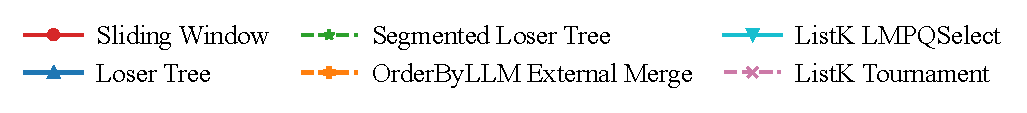
\includegraphics[width=0.88\linewidth]{fig/panels/exp2/exp2_legend.pdf}

  \vspace{-0.3em}

  \subfigure[\Movies (Token)]{
      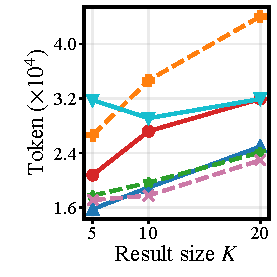
\includegraphics[width=0.33\columnwidth]{fig/panels/exp2/exp2_movies_tokens.pdf}
  }
  \hspace{-2.5ex}
  \subfigure[\Movies (Latency)]{
      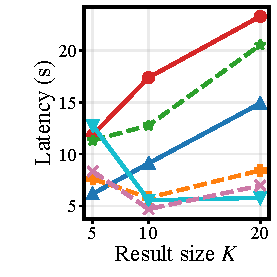
\includegraphics[width=0.33\columnwidth]{fig/panels/exp2/exp2_movies_latency.pdf}
  }
  \hspace{-2.5ex}
  \subfigure[\Movies (nDCG)]{
      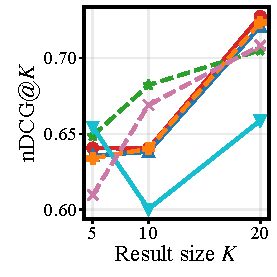
\includegraphics[width=0.33\columnwidth]{fig/panels/exp2/exp2_movies_quality.pdf}
  }

  \subfigure[\DLtwozero (Token)]{
      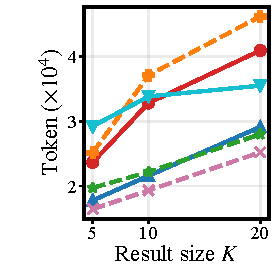
\includegraphics[width=0.33\columnwidth]{fig/panels/exp2/exp2_dl20_tokens.pdf}
  }
  \hspace{-2.5ex}
  \subfigure[\DLtwozero (Latency)]{
      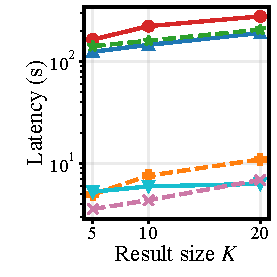
\includegraphics[width=0.33\columnwidth]{fig/panels/exp2/exp2_dl20_latency.pdf}
  }
  \hspace{-2.5ex}
  \subfigure[\DLtwozero (nDCG)]{
      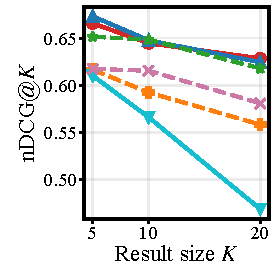
\includegraphics[width=0.33\columnwidth]{fig/panels/exp2/exp2_dl20_quality.pdf}
  }

  \caption{Sensitivity of token cost, latency and nDCG@$K$ in \LIMIT~$K$  by varying $K\in\{5,10,20\}$ ($m{=}10$)}
  \label{fig:exp2-k}
\end{figure}

\Cref{tab:exp1-topk} reports the performance results of \LIMIT~$K$ at $K{=}10$ with the pipeline execution of \cref{sec:topk-exec}. All algorithms retain the default configuration from \cref{sec:exp:full}, isolating the effect of demand-driven execution. \Cref{fig:exp2-k} presents the impact of varying $k$. We evaluate ranking quality (nDCG@10), token cost ($\times 10^3$), and latency (seconds) across six benchmarks: \Movies, \DLtwozero, \DLtwotwo, \COVID, \Touche, and \FiQA. The comparison spans three categories of baselines: pointwise methods (Pointwise, Ext. Pointwise), bubble-based extensions (Ext. Bubble, Ext. Merge), and tournament-style selectors (LMPQSelect, Tournament), against our proposed demand-driven algorithms (\SD, \LT, \SLT).

\noindent \textbf{Quality and efficiency.} Our three algorithms consistently dominate in ranking quality. They claim the top three positions on \DLtwozero, \DLtwotwo, \Touche, and \FiQA; on \Movies, \SD and \LT tie for second. On \COVID they trail only Ext. Bubble and Tournament yet surpass all other baselines. Ext. Bubble and Tournament use acceptance criteria that require repeated comparisons before emitting an item, exposing top-ranked candidates to more competitors and trading higher cost for higher quality. In efficiency, \LT and \SLT match LMPQSelect in token cost while halving that of Ext. Bubble. Demand-driven execution yields dramatic reductions: \LT cuts token consumption by $3$--$5\times$ and latency by $4$--$9\times$ relative to full ranking, as the producer tree propagates only the requested prefix and overlaps adjacent levels without materializing intermediate runs.

\noindent \textbf{The bubble cost-quality trade-off.} Ext. Bubble achieves the highest nDCG on \COVID and strong results elsewhere, but its exhaustive pairwise comparisons incur prohibitive token costs—roughly double those of our \LT variants and an order of magnitude above pointwise methods. This confirms that bubble-based refinement, while accurate, does not scale efficiently.

\noindent \textbf{The pointwise cost-quality trade-off.} Pointwise and Ext. Pointwise minimize token expenditure and latency; Ext. Pointwise even achieves the best average rank in runtime. However, their nDCG scores fall markedly below all competing methods across every dataset. The gap is particularly severe on long-document collections such as \Touche. These results corroborate that pointwise formulations, despite their computational thrift, fail to capture the nuanced relevance signals required for high-quality ranking.

\subsection{Effectiveness of Segmented Loser Tree}
\label{sec:exp:ablation}

% Approved: PR4 cursor/e3-scale-layout-14e8
\begin{figure*}[t]
  \centering
  \includegraphics[width=178mm]{e3-scale.pdf}
  \caption{Synthetic layout for the fixed-$(k,h)$ scale figure, not a measured result.
  The contract names Qwen3.5-9B and one DL20 query; no run produced these heights.
  Input size $n$ is linear at 1k, 5k, and 10k. A logarithmic axis was not specified.
  Each color is one confirmed pair and is the same in the Full and LIMIT~10 panels of that family.
  A solid line with filled circles stands in for a measurement.
  A dashed line stands in for a prediction: the same scaffold plus a constant offset, not a model error.
  Vertical order follows the confirmed list and is not a ranking.
  Open stars are the four LT supplements and are not joined to the five series.
  Full uses $(250,2)$ at 5k and $(500,2)$ at 10k.
  LIMIT~10 uses $(250,1)$ at 5k and $(500,1)$ at 10k.
  Those stars are not per-size optima.
  The vertical unit is a layout unit, not tokens and not a cost.
  Cache off/on is not split, and per-size best $(k,h)$ are omitted.
  Legacy ablation panels in \cref{fig:exp3-ablation} remain until measured results replace them.}
  \label{fig:exp3-scale}
\end{figure*}

\begin{figure}[t]
  \centering

  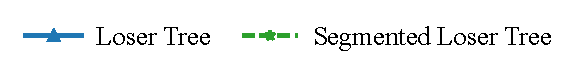
\includegraphics[width=0.65\linewidth]{fig/panels/exp3/exp3_legend.pdf}

  \vspace{-2.0ex}

  \subfigure[\Movies (full rank)]{
      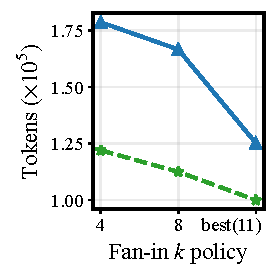
\includegraphics[width=0.33\columnwidth]{fig/panels/exp3/exp3_movies_full_tokens.pdf}
  }
  \hspace{-2.5ex}
  \subfigure[\Movies (full rank)]{
      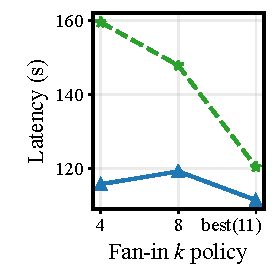
\includegraphics[width=0.33\columnwidth]{fig/panels/exp3/exp3_movies_full_latency.pdf}
  }
  \hspace{-2.5ex}
  \subfigure[\Movies (full rank)]{
      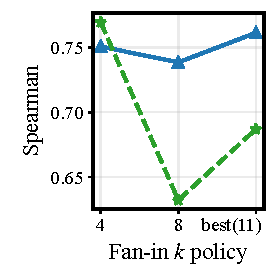
\includegraphics[width=0.33\columnwidth]{fig/panels/exp3/exp3_movies_full_quality.pdf}
  }

  \subfigure[\Movies (\LIMIT~10)]{
      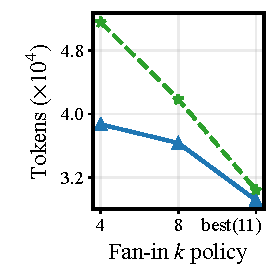
\includegraphics[width=0.33\columnwidth]{fig/panels/exp3/exp3_movies_top10_tokens.pdf}
  }
  \hspace{-2.5ex}
  \subfigure[\Movies (\LIMIT~10)]{
      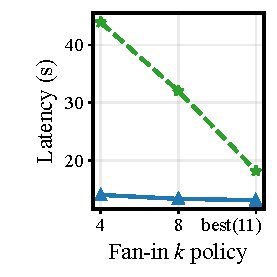
\includegraphics[width=0.33\columnwidth]{fig/panels/exp3/exp3_movies_top10_latency.pdf}
  }
  \hspace{-2.5ex}
  \subfigure[\Movies (\LIMIT~10)]{
      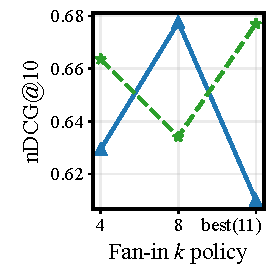
\includegraphics[width=0.33\columnwidth]{fig/panels/exp3/exp3_movies_top10_quality.pdf}
  }

  \subfigure[\DLtwozero (full rank)]{
      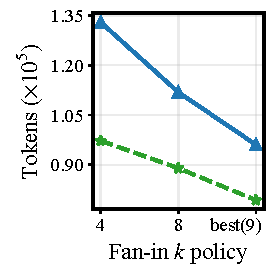
\includegraphics[width=0.33\columnwidth]{fig/panels/exp3/exp3_dl20_full_tokens.pdf}
  }
  \hspace{-2.5ex}
  \subfigure[\DLtwozero (full rank)]{
      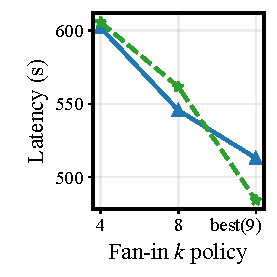
\includegraphics[width=0.33\columnwidth]{fig/panels/exp3/exp3_dl20_full_latency.pdf}
  }
  \hspace{-2.5ex}
  \subfigure[\DLtwozero (full rank)]{
      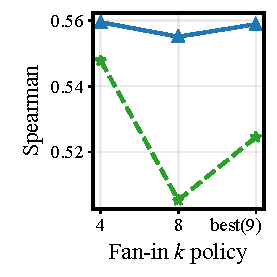
\includegraphics[width=0.33\columnwidth]{fig/panels/exp3/exp3_dl20_full_quality.pdf}
  }

  \subfigure[\DLtwozero (\LIMIT~10)]{
      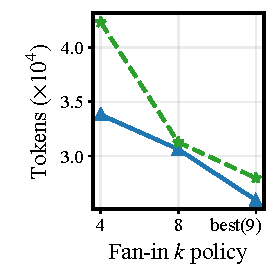
\includegraphics[width=0.33\columnwidth]{fig/panels/exp3/exp3_dl20_top10_tokens.pdf}
  }
  \hspace{-2.5ex}
  \subfigure[\DLtwozero (\LIMIT~10)]{
      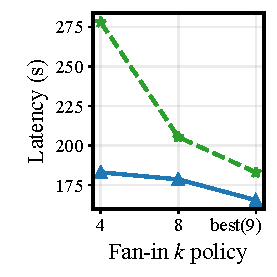
\includegraphics[width=0.33\columnwidth]{fig/panels/exp3/exp3_dl20_top10_latency.pdf}
  }
  \hspace{-2.5ex}
  \subfigure[\DLtwozero (\LIMIT~10)]{
      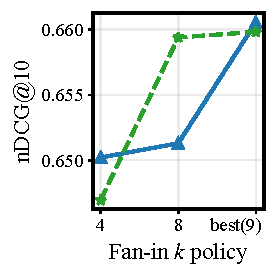
\includegraphics[width=0.33\columnwidth]{fig/panels/exp3/exp3_dl20_top10_quality.pdf}
  }

  \caption{Loser tree vs.\ segmented loser tree under fixed fan-in $k\in\{4,8\}$ and the choice from their cost models}
  \label{fig:exp3-ablation}
\end{figure}
\Cref{fig:exp3-ablation} isolates the effect of segmentation on \Movies and \DLtwozero under both full ranking and \LIMIT~10 settings. \SLT improves listwise throughput by emitting multiple items per listwise call while preserving the global ordering invariant. \SLT improves listwise throughput and consistently reduces token cost by 20\% on average, while latency and ranking quality remain comparable.

\noindent \textbf{Effectiveness of segmentation under \LIMIT~10.}
As \LT emits one item per listwise call, its pipelined merge stops as soon as the requested prefix is complete, avoiding listwise calls on unneeded items. 
Consequently, segmentation is counterproductive under \LIMIT~10: it increases both token cost and latency without a corresponding gain in nDCG.
For both \LT and \SLT on the two datasets, the fan-in $k$ selected by our cost model yields the lowest full ranking token cost. 
We further validate this selection in \cref{sec:exp:cost}.

\subsection{Cost Model Validation}
\label{sec:exp:cost}

% Approved: PR2 cursor/e2-dual-surface-c6cc commit 84a84ad (2x2 main text)
\begin{figure*}[t]
  \centering
  \includegraphics[width=\textwidth]{e2-layout-2x2.pdf}
  \caption{Synthetic layout preview for predicted vs.\ measured token-cost surfaces, not experimental results.
  Blue is measured and orange is predicted.
  Every panel uses the same camera.
  The predicted minimum is drawn at that configuration's measured height; a star on a diamond is both roles at one height.
  Missing corners are left empty.
  The SW column uses the SW legal window ($k\le 20$, $h\le m/k$); the LT column uses the LT window ($k\le 25$, $h$ bounded by max-segment).
  Full and LIMIT10 of one algorithm share that window, including the $z$ ticks.
  The two algorithms are not forced onto one numeric range.
  Panel assignment is not chosen.}
  \label{fig:exp2-surface-2x2}
\end{figure*}

\begin{figure*}[t]
  \centering

  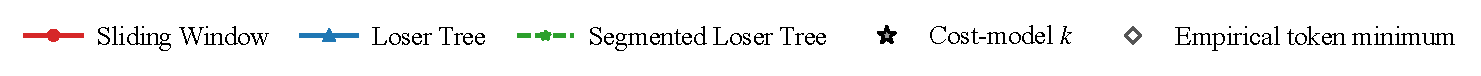
\includegraphics[width=0.75\linewidth]{fig/panels/exp4/exp4_legend.pdf}

  \vspace{-2ex}

  \subfigure[\Movies ($m{=}8$)]{
      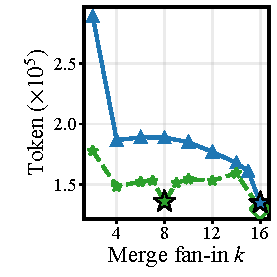
\includegraphics[width=0.33\columnwidth]{fig/panels/exp4/exp4_lt_movies_m8_tokens.pdf}
  }
  \hspace{-2.5ex}
  \subfigure[\DLtwozero ($n ={200}, m{=}10$)]{
      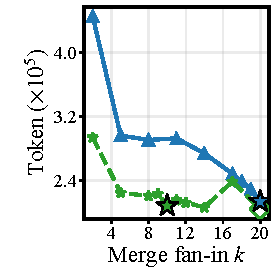
\includegraphics[width=0.33\columnwidth]{fig/panels/exp4/exp4_lt_dl20t200_m10_tokens.pdf}
  }
  \hspace{-2.5ex}
  \subfigure[\DLtwozero ($n{=}500, m{=}12$)]{
      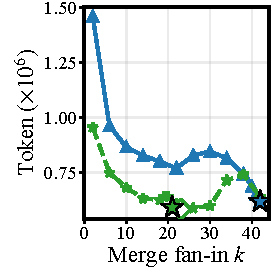
\includegraphics[width=0.33\columnwidth]{fig/panels/exp4/exp4_lt_dl20t500_m12_tokens.pdf}
  }
  \subfigure[\Movies ($m{=}8$)]{
      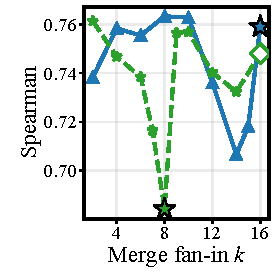
\includegraphics[width=0.33\columnwidth]{fig/panels/exp4/exp4_lt_movies_m8_quality.pdf}
  }
  \hspace{-2.5ex}
  \subfigure[\DLtwozero ($n{=}200, m{=}10$)]{
      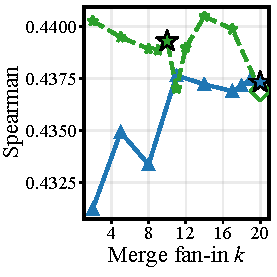
\includegraphics[width=0.33\columnwidth]{fig/panels/exp4/exp4_lt_dl20t200_m10_quality.pdf}
  }
  \hspace{-2.5ex}
  \subfigure[\DLtwozero ($n{=}500,m{=}12$)]{
      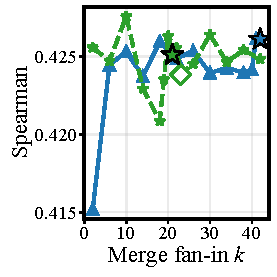
\includegraphics[width=0.33\columnwidth]{fig/panels/exp4/exp4_lt_dl20t500_m12_quality.pdf}
  }

  \subfigure[\Movies ($m{=}12$)]{
      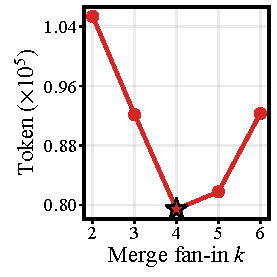
\includegraphics[width=0.33\columnwidth]{fig/panels/exp4/exp4_sw_movies_m12_tokens.pdf}
  }
  \hspace{-2.5ex}
  \subfigure[\DLtwozero ($n{=}500,m{=}20$)]{
      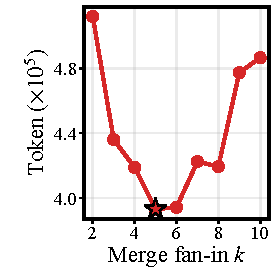
\includegraphics[width=0.33\columnwidth]{fig/panels/exp4/exp4_sw_dl20t500_m20_tokens.pdf}
  }
  \hspace{-2.5ex}
  \subfigure[\DLtwozero ($n{=}500, m{=}30$)]{
      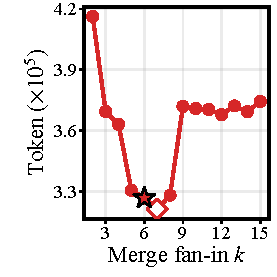
\includegraphics[width=0.33\columnwidth]{fig/panels/exp4/exp4_sw_dl20t500_m30_tokens.pdf}
  }
  \subfigure[\Movies ($m{=}12$)]{
      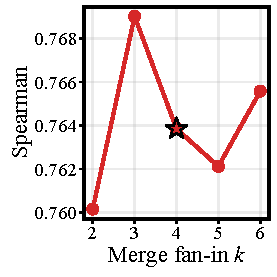
\includegraphics[width=0.33\columnwidth]{fig/panels/exp4/exp4_sw_movies_m12_quality.pdf}
  }
  \hspace{-2.5ex}
  \subfigure[\DLtwozero ($n{=}500,m{=}20$)]{
      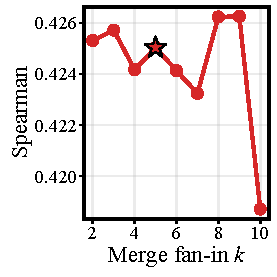
\includegraphics[width=0.33\columnwidth]{fig/panels/exp4/exp4_sw_dl20t500_m20_quality.pdf}
  }
  \hspace{-2.5ex}
  \subfigure[\DLtwozero($n{=}500, m{=}30$)]{
      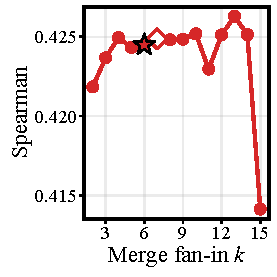
\includegraphics[width=0.33\columnwidth]{fig/panels/exp4/exp4_sw_dl20t500_m30_quality.pdf}
  }

  \caption{Cost model validation: Stars mark the cost model-selected $k_{\mathrm{sel}}$ and diamonds mark the empirical token minimum $k$.}
  \label{fig:exp4-full}
\end{figure*}

\begin{figure}[t]
  \centering

  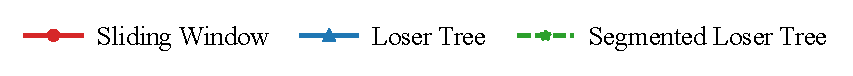
\includegraphics[width=0.88\linewidth]{fig/panels/exp4/exp4_topk_legend.pdf}

  \vspace{-0.4em}

  \subfigure[\Movies]{
      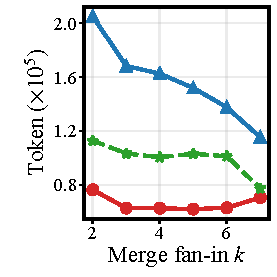
\includegraphics[width=0.25\columnwidth]{fig/panels/exp4/exp4_topk_movies_m20_tokens.pdf}
  }
  \hspace{-2.6ex}
  \subfigure[\Movies ]{
      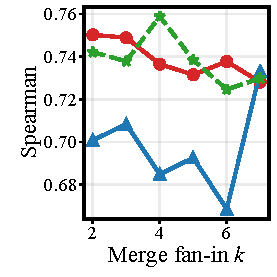
\includegraphics[width=0.25\columnwidth]{fig/panels/exp4/exp4_topk_movies_m20_quality.pdf}
  }
\hspace{-2.6ex}
  \subfigure[\DLtwozero]{
      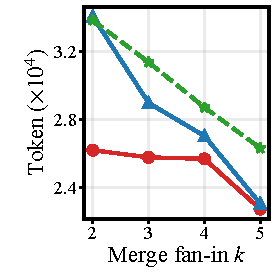
\includegraphics[width=0.25\columnwidth]{fig/panels/exp4/exp4_topk_dl20_m20_tokens.pdf}
  }
  \hspace{-2.6ex}
  \subfigure[\DLtwozero]{
      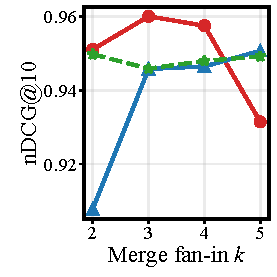
\includegraphics[width=0.25\columnwidth]{fig/panels/exp4/exp4_topk_dl20_m20_quality.pdf}
  }

  \caption{Sensitivity of fan-in $k$ under \LIMIT~10}
  \label{fig:exp4-topk}
\end{figure}

\begin{figure*}[t]
  \centering

  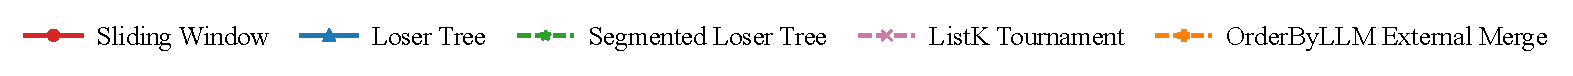
\includegraphics[width=0.8\linewidth]{fig/panels/exp5/exp5_legend.pdf}

  \vspace{-2ex}

  \subfigure[\Movies (full rank)]{
      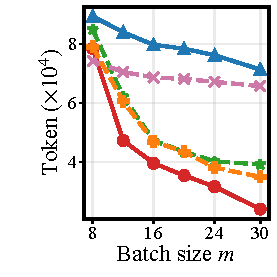
\includegraphics[width=0.33\columnwidth]{fig/panels/exp5/exp5_movies_full_tokens.pdf}
  }
  \hspace{-2.5ex}
  \subfigure[\Movies (full rank)]{
      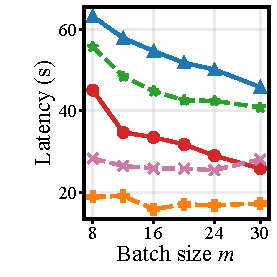
\includegraphics[width=0.33\columnwidth]{fig/panels/exp5/exp5_movies_full_latency.pdf}
  }
  \hspace{-2.5ex}
  \subfigure[\Movies (full rank)]{
      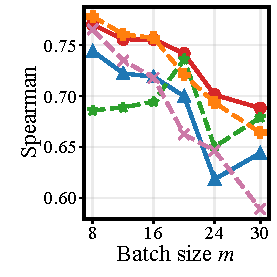
\includegraphics[width=0.33\columnwidth]{fig/panels/exp5/exp5_movies_full_quality.pdf}
  }
  \subfigure[\Movies (\LIMIT~$10$)]{
      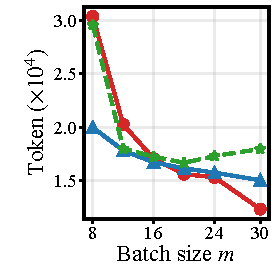
\includegraphics[width=0.33\columnwidth]{fig/panels/exp5/exp5_movies_top10_tokens.pdf}
  }
  \hspace{-2.5ex}
  \subfigure[\Movies (\LIMIT~$10$)]{
      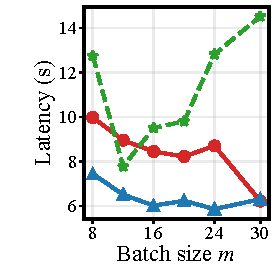
\includegraphics[width=0.33\columnwidth]{fig/panels/exp5/exp5_movies_top10_latency.pdf}
  }
  \hspace{-2.5ex}
  \subfigure[\Movies (\LIMIT~$10$)]{
      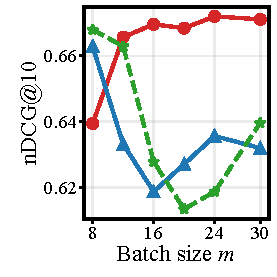
\includegraphics[width=0.33\columnwidth]{fig/panels/exp5/exp5_movies_top10_quality.pdf}
  }

  \subfigure[\DLtwozero (full rank)]{
      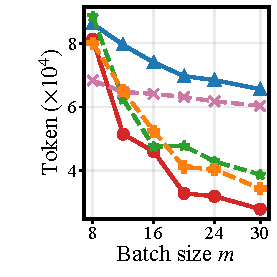
\includegraphics[width=0.33\columnwidth]{fig/panels/exp5/exp5_dl20_full_tokens.pdf}
  }
  \hspace{-2.5ex}
  \subfigure[\DLtwozero (full rank)]{
      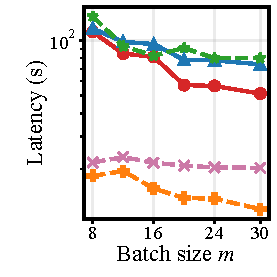
\includegraphics[width=0.33\columnwidth]{fig/panels/exp5/exp5_dl20_full_latency.pdf}
  }
  \hspace{-2.5ex}
  \subfigure[\DLtwozero (full rank)]{
      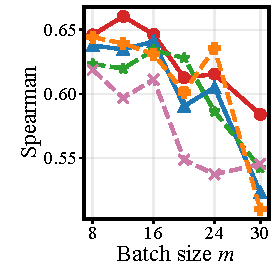
\includegraphics[width=0.33\columnwidth]{fig/panels/exp5/exp5_dl20_full_quality.pdf}
  }
  \subfigure[\DLtwozero (\LIMIT~$10$)]{
      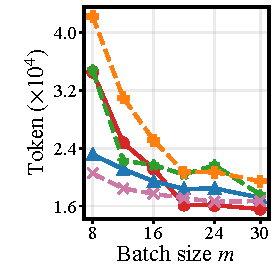
\includegraphics[width=0.33\columnwidth]{fig/panels/exp5/exp5_dl20_top10_tokens.pdf}
  }
  \hspace{-2.5ex}
  \subfigure[\DLtwozero (\LIMIT~$10$)]{
      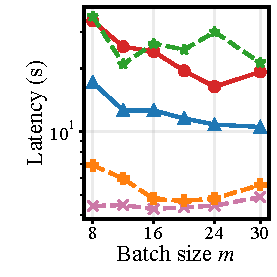
\includegraphics[width=0.33\columnwidth]{fig/panels/exp5/exp5_dl20_top10_latency.pdf}
  }
  \hspace{-2.5ex}
  \subfigure[\DLtwozero (\LIMIT~$10$)]{
      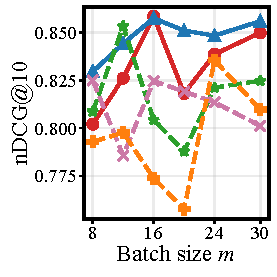
\includegraphics[width=0.33\columnwidth]{fig/panels/exp5/exp5_dl20_top10_quality.pdf}
  }

  \caption{Impact of listwise batch size $m$ on cost, latency and quality}
  \label{fig:exp5-m}
\end{figure*}


We evaluate the impact of fan-in $k$ on token cost and ranking quality for our three algorithms across three datasets.
For each algorithm, we sweep $k$ at two fixed batch sizes $m$, with both full ranking and \textsc{Limit}~$K{=}10$. 
For full ranking, we mark the cost-model-selected $k_a^\star$ on each sweep curve. 
Results show $k_a^\star$ precisely matches with the empirical token optimum $k^*$ or lies near it. $k_a^\star=k^*$ occurs in five of all six settings, with the remaining mismatched setting's token regret at most $1.99\%$. 
This confirms our cost model effectively selects the cost-optimal $k$.

\noindent \textbf{Token cost vs.\ fan-in.}
\LT exhibits monotonically decreasing token cost as $k$ increases, reaching minimum at $k=r$. In contrast, \SD and \SLT show U-shaped curves: cost first decreases then increases with $k$, yielding an interior minimum. For \SD, this reflects the trade-off between fewer merge rounds (larger $k$) and higher per-round prompt complexity. \SLT balances larger segments against segmented structure overhead. The per-pass cost of \LT is nearly independent of $k$, which is deduced in~\cref{subsec:cost-loser-tree}, so minimizing the number of passes is optimal, with $k{=}r$ completing the merge in one pass. On \Movies at $m{=}8$, the selected fan-in saves $27.8\%$ for \LT and $8.5\%$ for \SLT relative to $k{=}4$; \SD saves $21.5\%$--$24.6\%$ relative to $k{=}2$. Larger deviations at $m{=}8$ occur in narrow feasible ranges.

\noindent \textbf{Ranking quality vs.\ fan-in.}
Fan-in affects quality far less than cost. At selected $k_a^\star$, quality remains close to the best measured value in all settings except \LT on \Movies at $m{=}8$. Quality curves show no consistent trend with $k$, indicating cost-driven selection introduces no systematic quality loss. Thus optimizing $k$ for token cost preserves ranking effectiveness.


\subsection{LIMIT $n$ sensitivity (layout integration)}
\label{sec:exp:limit-sweep}

% Parent-approved LIMIT-n sweep layouts (synthetic); does not replace fig:exp5-m.
% E5: Off + On-cold on one float page (proportional scale; aspect preserved).
\begin{figure*}[t]
  \centering
  \subfigure[Cache Off (\(\beta{=}0\), \(U\) cost scale).]{%
    \includegraphics[width=\linewidth,height=0.38\textheight,keepaspectratio]{e5-limit-sweep-off.pdf}%
    \label{fig:exp5-k-sweep-off}}%
  \subfigure[Cache On-cold (measured \(U{-}Q\) scale).]{%
    \includegraphics[width=\linewidth,height=0.38\textheight,keepaspectratio]{e5-limit-sweep-on.pdf}%
    \label{fig:exp5-k-sweep-on}}%
  \caption{Synthetic layout---not experimental results. LIMIT~$n$ contract: equal category spacing (not linear in $n$); Full isolated; LIMIT~500 is last connected point.}
\end{figure*}

\subsection{Impact of Listwise Batch Size}
\label{sec:exp:m}



\Cref{fig:exp5-m} studies the impact of the listwise batch size $m$ on token cost, latency, and ranking quality for both full-ranking and \LIMIT~10 workloads on \Movies and \DLtwozero.
Five merge algorithms are evaluated under the same batch sizes setting.
Overall, increasing $m$ exposes a clear trade-off between token cost and quality.
Larger batch size reduces the number of LLM invocations and token consumption, but they also make each invocation more difficult for the LLM.
As a result, full-ranking quality gradually deteriorates as $m$ increases, while latency exhibits a non-monotonic trend because the reduction in invocation count competes with the increasing cost of each individual LLM call.


\noindent \textbf{Impact of batch size $m$ on token cost and quality.}
Increasing $m$ consistently reduces token cost across all algorithms.
The reason is straightforward: a larger listwise batch ranks more items in each LLM invocation, thereby reducing both the number of initial runs ($r=\lceil n/m\rceil$) and the subsequent merge operations.
This reduction in token cost comes at the expense of ranking quality.
As $m$ grows, each LLM call must jointly order more candidates within a single context, making the ranking task increasingly challenging and introducing more ordering errors.
These errors accumulate throughout the merge process and are reflected by the full-ranking Spearman metric.
In contrast, \LIMIT~10 remains relatively stable because only the highest-ranked items are evaluated, making errors in the tail of the ranking largely invisible.


\noindent \textbf{Impact of batch size $m$ on latency.}
The effect of $m$ on latency is more nuanced.
Increasing $m$ reduces the number of LLM invocations almost linearly, which tends to lower the overall execution time.
However, each invocation becomes substantially more expensive because a larger batch produces a longer prompt and requires the LLM to reason over more candidates simultaneously.
The computational cost of Transformer attention increases superlinearly with the input length during prompt processing, while longer prompts also increase the amount of decoding tokens.
Consequently, the increased latency of each individual call can offset, or even outweigh, the reduction in invocation count.


\section{Related Work}
\label{sec:relatedwork}

\stitle{Semantic query processing.}
LOTUS exposes semantic operators in a dataframe interface and develops execution strategies for operators such as filtering, joins, and top-$K$ ranking~\cite{DBLP:journals/pvldb/PatelJPGAGZ25}.
Unify organizes analytics over unstructured data as pipelines of semantic operators~\cite{DBLP:journals/pvldb/WangLWXL25}.
Other systems use inexpensive proxy models to reduce the number of LLM calls needed to evaluate semantic predicates~\cite{DBLP:journals/pacmmod/ZeighamiSP25,DBLP:journals/corr/abs-2509-12610,DBLP:journals/corr/abs-2601-05536}.
In semantic \textsf{ORDER BY}, the placement of a row also depends on the other rows. A bounded prompt therefore determines not only how many rows an operator can inspect, but also which relative orders it can establish together.

\stitle{LLM ranking and external merge.}
Pointwise ranking scores items independently~\cite{DBLP:conf/emnlp/DrozdovZD0RWAIM23,DBLP:conf/emnlp/SachanLJAYPZ22}, while pairwise methods aggregate comparisons between items~\cite{DBLP:conf/acl/LuoCH024,DBLP:conf/naacl/QinJHZWYSLLMWB24}.
Listwise ranking compares a slate in a single prompt, and setwise ranking can select a preferred item from a set~\cite{DBLP:conf/sigir/ZhuangZKZ24,DBLP:conf/emnlp/0001YMWRCYR23,DBLP:journals/corr/abs-2305-02156}.
ListK uses listwise tournament and multi-pivot operators for selection and sorting~\cite{DBLP:journals/corr/abs-2603-17223}.
Zhao et al. generate sorted runs and combine them by two-way external merge~\cite{DBLP:journals/corr/abs-2509-00303}.
We build on the external sorting abstraction~\cite{DBLP:journals/csur/Graefe06} and study what happens inside and between merge groups. A group can reuse a ranked window or refresh a single tree path, and the choice of fan-in and buffer capacity changes both the prompt contents and the amount of work needed to meet the requested output.

\section{Conclusion}
\label{sec:conclusion}
Semantic \textsf{ORDER BY} must assemble a global ranking from listwise calls that can see only part of the input. Our framework organizes these calls as external $k$-way merge. Sliding windows carry uncommitted items between calls, and segmented loser trees replace one segment along the path that next needs input. The same merge groups support full ranking through layer materialization and \LIMIT~$K$ through demand-driven execution. By accounting for both calls and repeated item appearances, the planner can choose the merge family, fan-in, and capacity for the requested output.

\FloatBarrier
\bibliographystyle{vendor/ACM-Reference-Format}
\bibliography{ref}
\clearpage
\appendix
\section{Algorithm Correctness}
\label{app:algorithm-proofs}

For the sortedness results, fix a strict total order $\prec$ on row identities for instruction $\phi$, with one tie-breaking rule across calls. A \emph{consistent oracle} returns the restriction of $\prec$ to its input batch. A weaker contract, used in Section~\ref{app:proof-inconsistent}, requires only that each rank call supply a permutation of its input. In either case, two rows with identical contents are still distinct identities.

\subsection{Sliding-Window Merge}
\label{app:proof-sw}

\begin{lemma}[Safe window prefix]
For runs sorted by $\prec$ and a consistent oracle, each round of Algorithm~\ref{alg:sliding_window_kway_group_merge} emits a nonempty prefix of the sorted union of the outstanding rows whenever any row remains. Its rank batch has at most $gh$ rows.
\end{lemma}
\begin{proof}
After refill, the buffered rows from each run form a contiguous prefix of its remaining rows. This holds initially and will be preserved if a round removes a prefix from each run. For each run $u$ with an unread suffix, let $z_u$ be its last buffered row. Such a row exists because $h\ge1$ and refill reads until the quota is met or the source is exhausted. Let $j_u$ be the position of $z_u$ in the oracle order $O$. The round emits up to $t=\min_u j_u$, or all of $O$ if no unread suffix remains.

Each emitted row occurs at or before $z_u$ in $O$ for every such $u$. Since every unread row of $u$ follows $z_u$ in $\prec$, no unread row precedes any emitted row. The emitted prefix also precedes all buffered survivors. Its restriction to each run is therefore a prefix, establishing the invariant for the next round. A fully exposed run, including a short final run, imposes no boundary. With a single live run, its buffer followed by its unread suffix is already in order. Each round with remaining rows makes progress, and each of the $g$ buffers holds at most $h$ rows.
\end{proof}

\subsection{Segmented Loser-Tree Merge}
\label{app:proof-lt}

For a node $v$, let its two child streams deliver blocks of $h$ rows, except for a possibly short block at exhaustion. Each replay slot is associated with one child. Its \emph{frontier} is the maximum real row in the slot if the slot is full, and $+\infty$ otherwise. The slot need not consist of rows from its associated child.

\begin{lemma}[Node replay]
Before replay, suppose the slots hold exactly the rows fetched by $v$ but not yet forwarded. For each child, all rows not yet fetched from it follow the frontier of its slot. If a slot has frontier $+\infty$, that child is exhausted. Algorithm~\ref{alg:replay_segment_node} emits the next block in $\prec$ and restores this invariant when the pointed child supplies its next block.
\end{lemma}
\begin{proof}
Initially each slot is a block from its own child, so the frontier condition follows from child order. When the two slots are ranked together, let $b_L,b_R$ denote their frontiers. If a child has unread rows, its slot contains $h$ rows no later than its frontier. The first $h$ rows of the union are therefore no later than the frontier of either child with unread rows. They precede every unread row. If the union has fewer than $h$ rows, both slots are short and neither child has unread rows. In either case, the winner contains exactly the next block.

After padding, the first slot to contribute its $h$-th entry is the one with the smaller frontier; if both frontiers are infinite, either child is already exhausted. The retained loser holds all real rows not forwarded from the slots. If both slots were full, the loser has size $h$ and contains the larger frontier. If either slot was short, the loser is short and the unpointed child has infinite frontier. Hence the loser inherits the frontier of the unpointed child even when its rows came from both children. A fresh block from the pointed child restores its own frontier. This proves the invariant by induction. For example, with $h=2$ and slots $[1,100]$ and $[3,4]$, replay emits $[1,3]$, retains $[4,100]$, and refills the second slot.
\end{proof}

\begin{lemma}[Tree construction and path refresh]
Algorithms~\ref{alg:loser_tree_kway_group_merge} and~\ref{alg:refresh_loser_tree_path} implement this node rule over the entire halving tree. For input runs sorted by $\prec$ and a consistent oracle, they return their sorted union.
\end{lemma}
\begin{proof}
View each internal node as a producer whose first block comes from the first replay of its two child blocks. To obtain its next block, it requests the next block only from its pointed child. Starting at the root, these requests form one descending path. The leaf supplies a fresh block, and replays on the return path rebuild the winner, loser, and pointer at each visited node. Every node off the path receives no request, so its stored state remains valid.

Within a packed initialization block or a refresh path, a replay sees only subsets of the ranked batch: all incoming winners are composed of its rows. With a consistent oracle, restricting the shared rank map to any such subset gives exactly the same order as ranking that subset alone. The run-order repair also leaves a consistent rank map unchanged. Thus the packed build and the fused refresh implement the same recursive producer, and induction on subtree height gives its sorted stream. Virtual rows never enter that stream or a prompt. Empty child blocks, short tails, and unequal path lengths are handled by the same invariant. If a group has one run, it forwards the run without a tree.

Each initialization batch contains at most $\lfloor m/h\rfloor$ frontier blocks by construction. For $g\ge2$ leaves the depth of the halving tree is $d=\lceil\log_2 g\rceil$: after $j$ levels a subtree has at most $\lceil g/2^j\rceil$ leaves, and a shallower binary tree cannot hold $g$ leaves. The quota bound implies $\lfloor m/h\rfloor\ge2$, so each frontier cut before the root can contract at least one pair of siblings in the contracted tree. A refresh sees at most $d$ losers and one replacement block, for at most $(d+1)h\le m$ real rows. For $h=1$ and a nonempty winner, the first slot to exhaust supplies the single winner, and the retained slot holds the opponent. The pointer then follows the winner's run as in a classical loser tree.
\end{proof}

\subsection{Materialization and Prefix Execution}
\label{app:proof-limit}

\begin{theorem}[Full ranking and LIMIT]
Under a consistent oracle, Algorithm~\ref{alg:semantic_external_merge} returns the $\prec$-sorted permutation for Full ranking ($K=\infty$) and its first $\min(K,n)$ rows for \textsf{LIMIT}~$K$, for any feasible plan of the stated form.
\end{theorem}
\begin{proof}
The phase-one calls produce sorted runs that partition the input by row identity. At each pass, the groups partition the current runs. The group lemmas and the singleton rule replace each group with its sorted union, preserving the partition and order invariant. Let $r_t$ be the number of runs after $t$ passes, with $r_0=r$. The recurrence $r_{t+1}=\lceil r_t/k\rceil$ gives $r_t=\lceil r/k^t\rceil$, so one sorted stream remains after $\lceil\log_k r\rceil$ passes when $r\ge1$. Empty inputs, zero demand, and a single initial run take the direct branches.

For demand-driven execution, fix a physical plan and consider any prefix request at a producer. By induction on the height of the physical merge tree, each child responds to a request for $q$ rows with the next $q$ rows, or all remaining rows if fewer remain. This contract collects partial deliveries until the demand is met or the child reports exhaustion. At the parent, each refill therefore receives the same next rows as it would from materialized input. Applying the group rule to these rows and keeping the unreturned portion of an emitted block gives the parent's next consecutive slice. Repeating this argument for successive requests yields the corresponding root prefix. The root need not ask for another block after it has returned $K$ rows.
\end{proof}

The execution argument also gives a separate guarantee without a consistent oracle: with the same initial runs and physical plan, if each reached rank call receives the same response as its counterpart at the same producer in Full, strict demand returns the prefix of that Full execution. This is a coupling of local calls, not their global order. Independent plan selection or different model responses need not yield the same prefix.

\subsection{Guarantees with Inconsistent Rank Calls}
\label{app:proof-inconsistent}

\begin{proposition}[Row identity and run order]
If each call returns a permutation of its batch, both mergers preserve row identities: Full returns every input identity once, and \textsf{LIMIT} neither creates nor repeats an identity. In the LT group merger, every output prefix restricts to a prefix of every input run in its original order, even when rank calls disagree. The basic SW group merger does not have this run-prefix property.
\end{proposition}
\begin{proof}
Both mergers move real rows without copying or dropping them. SW removes precisely the rows it emits and consumes at least one row in every nonempty round. In LT, replay partitions the real slots between the winner and loser. For termination we need only the exhaustion part of the slot invariant, not the ordering of the frontiers: initially a short slot means its child has ended. If exactly one slot is short, all entries of the full slot precede any padding, so the full slot is the one selected for refill and the short loser stays associated with the exhausted child. If both slots are full, the loser is full; if both are short, both children have ended. The condition is preserved on refill. Thus an empty winner implies no resident row and no unread child rows. By induction on height, a drained LT tree returns all its real rows. Physical groups have disjoint inputs, and partial output stops only at the root.

For the LT run-prefix claim, fix one input run $R$ of an LT group. All its rows enter any ancestor node through the same child, even after a cached segment is reassigned to a replay slot. Induct on node height and on the number of replays at each node. The child delivers the $R$-subsequence in run order, with no gaps. At a replay the $R$-rows already fetched but not yet forwarded are exactly the $R$-rows in the slots. LT repairs each rank map by admitting only the earliest remaining row from each run, so the replay order preserves the order of these rows. Selecting a prefix of the replay order can only forward the next rows of $R$, and it cannot skip an as-yet-unfetched row of $R$. The argument uses the child stream's order even when that child lies outside the current refresh path; a node not replayed retains its state. It applies to initialization and to any truncation of the root output. Across LT-only passes, projecting a prefix onto an intermediate run and then onto an initial run composes the same property.

In SW, take $R_1=(a_1,a_2,a_3,a_4)$, $R_2=(b_1,b_2)$, and $h=2$. The first call can rank the buffer as $(a_2,b_1,a_1,b_2)$. The window rule emits through $a_1$, and \textsf{LIMIT}~$2$ returns $(a_2,b_1)$ without $a_1$. Thus consuming a prefix of a ranked window does not enforce the order of its source runs.
\end{proof}

\section{Additional Cost-Model Analysis}
\label{app:cost-results}

\subsection{Exact Case for Single-Item Segments}

Let $\ell_i$ be the positive lengths of the initial runs, let $h=1$, and let $1\le K\le\min_i\ell_i$. Under uniform rank interleaving, initialization has deterministic counts $(A_0,S_0)$: every child can supply its first row and the packed cuts are fixed by the plan. Initialization produces the first root row and installs one outstanding head from each initial run. A head may be pending at the root or retained inside a merge group. With strict demand, each refresh replaces just the head emitted at the root, following its source through all merge groups on its path. Before any of the next $K-1$ outputs, fewer than $\ell_i$ rows of each run $i$ have been emitted, so the replacement exists and no opponent is missing. Hence one such step incurs the path counts $(a_i,d_i)$ defined in Section~\ref{sec:cost-limit}. Each position in a uniformly interleaved order has source $i$ with marginal probability $\ell_i/n$. Linearity of expectation for the $K-1$ preceding positions yields Eq.~\eqref{eq:cost-limit-single}; it does not require those positions to be independent. Once a source can run short or $h>1$, the estimator uses the finite execution trace.

\subsection{When Sliding-Window Prefixes Shorten}

At the first window, if the first $h$ ranks all come from one run with unread rows, SW stops after $h$ outputs. A more even interleaving can extend that prefix. The uniform model can thus overestimate the safe prefix when head ranks concentrate in one run. Later windows also depend on which rows survived earlier rounds. The simulator retains their assigned ranks, so it does not draw independent window orders. More Monte Carlo samples improve precision under the assumed interleaving; they do not correct a mismatch between that distribution and the workload.

\subsection{Calls Needed to Certify the First Row}

Consider $r$ nonempty sorted runs, no known cross-run order, and a consistent comparison oracle of capacity $m\ge2$. Join runs in a graph when a call ranks rows from both. If the graph is disconnected, any component could contain the first row without contradicting the observations. Each call reduces the component count by at most $m-1$, so certifying the first row needs at least $\lceil(r-1)/(m-1)\rceil$ calls. This is tight: starting with all run heads, replace $\min(m,c)$ of the $c$ remaining candidates by their winner until one remains.

\end{document}
